% \documentclass[a4paper, 12pt, oneside]{report} % for final draft compilation
\documentclass[a4paper, 12pt, oneside, draft]{report} % for draft compilation

% Preamble:
\usepackage[T1]{fontenc}                            % package for specifying output font encoding
\usepackage[utf8]{inputenc}                         % package for specifying input font encoding
\usepackage{natbib}                                 % package for reference management
\usepackage{graphicx}                               % package for graphics handling (i.e. figure images)
\usepackage{mathptmx}                               % package for Times New Roman font
\usepackage{chngcntr}                               % package for making continuous figure numbering, instead of section-based numbering
\usepackage[flushleft]{threeparttable}              % package to add notes at the bottom of the table
\usepackage{setspace}                               % package for setting line space (used in title page)
\usepackage[hidelinks, colorlinks]{hyperref}        % package for hyperlinking references - hidelinks option removes the ugly boxes around the huperlinks
\usepackage[md]{titlesec}                           % package for tweaking the chapter/section/subsection titles format
\usepackage[acronym, toc]{glossaries}               % package for making glossaries
\usepackage{xcolor,colortbl}                        % package for making colours
\usepackage[noabbrev,capitalise]{cleveref}          % package for referencing multiple referencing in a single \ref command
\usepackage[font=footnotesize,format=hang]{caption} % package for formatting figure caption

% Define colour(s) for table rows:
\definecolor{LightCyan}{rgb}{0.88,1,1}

% Set up the hyperlinks - change the colour of the links to blue:
% \hypersetup{allcolors=blue}
\hypersetup{allcolors=black} % uncomment this line to make the hyperlinks black

% Change the default cref name for equations:
\creflabelformat{equation}{#2\textup{#1}#3}

% Change the default url font:
\urlstyle{rm}

% change figure numbering from section-based to continuous:
\counterwithout{figure}{chapter}
\counterwithout{equation}{chapter}
\counterwithout{table}{chapter}

% Change the title of bibliography to references:
\renewcommand{\bibname}{References}

% Italicise the subsubsection title:
\titleformat{\subsubsection}{\normalfont\itshape\bfseries}{\thesubsubsection}{1em}{}
\titleformat{\paragraph}{\normalfont\itshape}{\theparagraph}{\noindent}{}

% For generating glossaries:
%%%%%%%%%%%%%%%%%%%%%%%%%%%%%%%%%%%%%%%%%%%%%%%%%%%%%%%%%%%%%%%%%%%%%%%%%%%%%%%
%% Glossary terms
%%%%%%%%%%%%%%%%%%%%%%%%%%%%%%%%%%%%%%%%%%%%%%%%%%%%%%%%%%%%%%%%%%%%%%%%%%%%%%%

% TODO: make sure you get a proper definitions for all of these glossary terms

\newglossaryentry{rnaseq}{
	name=RNA-seq,
	description={sequence data using transcriptome}
}

\newglossaryentry{r}{
	name=R,
	description={Statistical programming language}
}

\newglossaryentry{metagene}{
	name=Metagene,
	text=metagene,
	description={Summary score of a sample that represents the overall gene expression of the genes that was used to obtain the scores}
}

\newglossaryentry{ldp}{
	name=Limited duration prevalence,
	text=limited duration prevalence,
	description={Number of patients diagnosed with a disease within a fixed period of time in the past \citep{Bray2013}}
}

\newglossaryentry{apoptosis}{
	name=Apoptosis,
	text=apoptosis,
	description={The death of cells which occurs as a normal and controlled part of an organism's growth or development}
}

\newglossaryentry{chromothripsis}{
	name=Chromothripsis,
	text=chromothripsis,
	description={An all-at-once mutational pattern in which a large number of rearrangements are confined to local regions of one or more chromosomes \citep{Stephens2011}}
}

\newglossaryentry{kataegis}{
	name=Kataegis,
	text=kataegis,
	description={Showers of single nucleotide changes confined to local regions, often near sites of chromosome rearrangements \citep{Stephens2011}}
}

\newglossaryentry{adipocyte}{
	name=Adipocyte,
	text=adipo\-cyte,
	plural=adipo\-cytes,
	description={Adipose tissue cell}
}

%%%%%%%%%%%%%%%%%%%%%%%%%%%%%%%%%%%%%%%%%%%%%%%%%%%%%%%%%%%%%%%%%%%%%%%%%%%%%%%
%% Acronym terms
%%%%%%%%%%%%%%%%%%%%%%%%%%%%%%%%%%%%%%%%%%%%%%%%%%%%%%%%%%%%%%%%%%%%%%%%%%%%%%%

\newacronym{blca}{BLCA}{bladder urothelial carcinoma}
\newacronym{cesc}{CESC}{cervical squamous cell carcinoma and endocervical adenocarcinoma}
\newacronym{coad}{COAD}{colon adenocarcinoma}
\newacronym{kirp}{KIRP}{kidney renal clear cell carcinoma}
\newacronym{lihc}{LIHC}{liver hepatocellular carcinoma}
\newacronym{read}{READ}{rectum adenocarcinoma}
\newacronym{skcm}{SKCM}{skin cutaneous melanoma}
\newacronym{ucec}{UCEC}{uterine corpus endometrial carcinoma}
\newacronym{geo}{GEO}{Gene Expression Omnibus}
\newacronym{tcga}{TCGA}{The Cancer Genome Atlas}
\newacronym{icgc}{ICGC}{International Cancer Genome Consortium}
\newacronym{bmi}{BMI}{Body Mass Index}
\newacronym{who}{WHO}{World Health Organization}
\newacronym{ln}{LN}{lymph node}
\newacronym{pr}{PR}{progesterone receptor}
\newacronym{er}{ER}{estrogen receptor}
\newacronym{her2}{HER2}{human epidermal growth factor receptor 2}
\newacronym{svd}{SVD}{singular value decomposition}
\newacronym{rma}{RMA}{Robust Multi Array}
\newacronym{mas}{MAS5}{Microarray Analysis Suite 5.0}
\newacronym{fdr}{FDR}{False Discovery Rate}
\newacronym{go}{GO}{Gene Ontology}
\newacronym{usa}{USA}{United States of America}
\newacronym{npy}{NPY}{neuropeptide Y}
\newacronym{agrp}{AGRP}{agouti-related protein}
\newacronym{pomc}{POMC}{pro-opiomelanocortin}
\newacronym{cart}{CART}{cocaine and amphetamine related transcript}
\newacronym{mc1r}{MC1R}{melanocortin 1 receptor}
\newacronym{mc4r}{MC4R}{melanocortin 4 receptor}
\newacronym{msh}{MSH}{melanocyte-stimulating hormone}
\newacronym{nyr1}{Y1R}{neuropeptide Y1 receptor}
\newacronym{acth}{ACTH}{adrenocorticotropic hormone}
\newacronym{ghsr}{GHSR}{growth hormone secretagogue receptor}
\newacronym{gaba}{GABA}{$\gamma$-aminobutyric acid}
\newacronym{irs}{IRS}{insulin receptor seubstrate}
\newacronym{pi3k}{PI3K}{phosphatidylinositol 3-kinase}
\newacronym{jak}{JAK}{janus kinase}
\newacronym{pc1}{PC1}{prohormone convertase 1}
\newacronym{fto}{FTO}{fat mass and obesity associated}
\newacronym{fto}{FTO}{fat mass and obesity associated}
\newacronym{snp}{SNP}{single nucleotide polymorphism}
\newacronym{rb}{RB}{retinoblastoma-associated}
\newacronym{opa}{OPA}{obesity policy action}
\newacronym{g1}{G1}{Gap 1}
\newacronym{bcl2}{Bcl-2}{B-cell lymphoma 2}
\newacronym{bh3}{BH3}{Bcl-2 homology 3}
\newacronym{dna}{DNA}{deoxyribonucleic acid}
\newacronym{vegf}{VEGF}{vascular endothelial growth factor}
\newacronym{vegfa}{VEGF-A}{vascular endothelial growth factor-A}
\newacronym{tsp1}{TSP-1}{thrombospondin-1}
\newacronym{emt}{EMT}{endothelial-mesenchymal transition}
\newacronym{met}{MET}{mesenchymal-endothelial transition}
\newacronym{aid}{AID}{activation-induced cytidine deaminase}
\newacronym{apobec}{APOBEC}{apolipoprotein B mRNA editing enzyme, catalytic polypeptide-like}
\newacronym{nfkb}{NF-$\kappa$B}{nuclear factor $\kappa$B}
\newacronym{stat3}{STAT3}{signal transducer and activator of transcription 3}
\newacronym{il6}{IL-6}{interleukin-6}
\newacronym{il10}{IL-10}{interleukin-10}
\newacronym{atp}{ATP}{adenosine triphosphate}
\newacronym{pep}{PEP}{phosphoenol pyruvate}
\newacronym{mmr}{MMR}{mismatch repair}
\newacronym{mtor}{mTOR}{mammalian target of rapamycin}
\newacronym{ner}{NER}{nucleotide-excision repair}
\newacronym{ber}{BER}{base-excision repair}
\newacronym{uv}{UV}{ultraviolet}
\newacronym{pah}{PAH}{polycyclic aromatic hydrocarbon}
\newacronym{nnk}{NNK}{4-(methylnitrosamino)-1-(3-pyridyl)-1-butanone}
\newacronym{ros}{ROS}{reactive oxygen species}
\newacronym{cyp}{CYP}{cytochrome P450}
\newacronym{igf}{IGF}{insulin-like growth factor}
\newacronym{igfbp}{IGFBP}{insulin-like growth factor binding protein}
\newacronym{gpcr}{GPCR}{G-protein coupled receptor}
\newacronym{tlr}{TLR}{Toll-like receptor}
\newacronym{prr}{PRR}{pattern recognition receptor}
\newacronym{ssdna}{ssDNA}{single-stranded DNA}
\newacronym{erk}{ERK}{extracellular signal regulated kinase}
\newacronym{cdna}{cDNA}{complimentary DNA}
\newacronym{mrna}{mRNA}{messenger RNA}
\newacronym{ngs}{NGS}{next generation sequencing}
\newacronym{fc}{FC}{fold change}
\newacronym{ifny}{IFN-$\gamma$}{interferon-$\gamma$}
\newacronym{tgfb}{TGF-$\beta$}{transforming growth factor-$\beta$}
\newacronym[longplural={genome wide association studies},\glsshortpluralkey={GWAS}]{gwas}{GWAS}{genome wide association study}
\newacronym{stat}{STAT}{signal transducer and activator of transcription}
\newacronym{pyy}{PYY$_{3-36}$}{peptide YY$_{3-36}$}
\newacronym[longplural={Disability-Adjusted Life Years}]{daly}{DALY}{Disability-Adjusted Life Year}


\makeglossaries

% Specify graphics path:
\graphicspath{ {./images/}}
\DeclareGraphicsExtensions{.pdf,.png,.jpg}

% If you want to compile specific files, uncomment the line below and add the filenames in the {} :
%\includeonly{}

\begin{document}

\include{./misc/title}

\pagenumbering{roman} % set page numbering to roman numeral

% Set line spacing to double space:
\onehalfspacing

%%%%%%%%%%%%%%%%%%%%%%%%%%%%%%%%%%%%%%%%%%%%%%%%%%%%%%%%%%%%
% Abstract for my thesis
%%%%%%%%%%%%%%%%%%%%%%%%%%%%%%%%%%%%%%%%%%%%%%%%%%%%%%%%%%%%
\vspace*{\fill}

\section*{\centering Abstract}
\addcontentsline{toc}{section}{Abstract}

Obesity has been a major global problem for more than a decade, associated with many noncommunicable diseases such as  cancer.
The number of obese people, in both adults and children, has risen in every country of the world and the trend will likely to continue in the future.
Cancers are caused by dysregulation of various molecular pathways that allow tumour cells to proliferate, survive and migrate.
One of the difficulties associated with the treatment of cancers is the identification of the underlying biological pathways that drive tumorigenesis.
This research aims to determine whether gene expression signatures exist  that are specific to obesity across multiple cancer types, and to investigate whether there are any common pathways being dysregulated in cancers based on these genetic signatures.
There were no genetic signatures or genes differentially expressed between obese and non-obese patients that were common across multiple cancer types.
However, the Akt, \gls{egfr} and Src pathways may have a role in promoting the tumour progression in patients that are obese.
It is likely that there is some complex mechanism underlying the relationship between obesity and cancer.
A better understanding of the pathways being dysregulated in cancer cells in obese patients may lead to improved clinical decisions, and contribute towards personalised treatment in the future.

\vfill


%%%%%%%%%%%%%%%%%%%%%%%%%%%%%%%%%%%%%%%%%%%%%%%%%%%%%%%%%%%%
% Acknowledgement for my thesis
%%%%%%%%%%%%%%%%%%%%%%%%%%%%%%%%%%%%%%%%%%%%%%%%%%%%%%%%%%%%

\vspace*{\fill}

\section*{\centering Acknowledgement}
\addcontentsline{toc}{section}{Acknowledgement}

First and foremost, I would like to thank my supervisor Mik, for giving me this project and an
opportunity to learn and develop the bioinformatics skills required to complete it.
You have been a great supervisor and I have learnt a lot from you over the past two years, and I have enjoyed being a part of the Black lab.
\\

\noindent
I would like to thank my committee members, Dr.\ Anita Dunbier, Dr.\ Miriam Sharpe, and Dr.\ Peter Mace (temporary member), for being patient during my presentations that were full of statistics and heatmaps.
I am grateful for all the suggestions and inputs you have given me to make this a better project.
\\

\noindent
I would also like to thank both past and present members of the Black lab, for useful tips and tricks to get me through my Masters.
Especially James Boocock, for introducing me to a variety of useful tool sets (by the way, everyone should start using vim); Murray Cadzow, for organising the fortnightly ``Shit You Should Know About'' (a.k.a. SYSKA) sessions to teach us more about R and other useful tools; and Tom Kelly, for being my companion in the Fish-bowl and helping me out with some of the code in my project.
\\

\noindent
I would like to thank all of my friends and family, for all their support and fun memories throughout the years that I have been at University.
I wish I could name everyone, but I don't think it's a good idea to extend this thesis any longer\ldots{}
Long story short, my life would not be nearly as interesting or enjoyable without you guys.
\\

\noindent
Lastly, a special thanks to Gezza and Tessa who generously proof-read my introduction.
\\

\vfill



\tableofcontents

\addcontentsline{toc}{section}{\contentsname}

\clearpage

\addcontentsline{toc}{section}{\listfigurename}

\listoffigures

\clearpage

\addcontentsline{toc}{section}{\listtablename}

\listoftables

\clearpage

\printglossaries

\clearpage

% \listoftables

% \clearpage

\pagenumbering{arabic} % revert the page numbering to normal numbering
\glsresetall

\chapter{Introduction (draft)}
\label{ch:intro}

\section{Obesity}
\label{sec:obesity}

Obesity has been one of the major global problems for more than a decade, associated with many noncommunicable diseases such as diabetes, cardiovascular diseases and certain types of cancers \citep{WHO2014}.
In fact, the risk of comorbidities increases with the increase in \gls{bmi}, where the risk becomes severe as the \gls{bmi} level approaches the obese category \citep{WHO2000}.

The number of overweight and obese people, in both adults and children, have risen in every country of the world, and the trend continues as we speak.
Estimated to account for 3.4 million deaths per year and 93.6 million \glspl{daly} in 2010, obesity is a serious disease that continues to grow in our society \citep{Lim2012}.

\subsection{Definition of obesity}
\label{sub:definition_of_obesity}

Obesity is defined as an abnormal or excessive fat accumulation that may impair health of that individual \citep{Garrow1988}.

One common and widely used approach to categorise individuals is by measuring the \gls{bmi} of the individual.
\gls{bmi} is a measurement based on the weight-to-height ratio of an individual that is used by clinicians and epidemiologists to classify adults into underweight, normal weight, overweight or obese categories.
The unit of \gls{bmi} is defined as the individual's weight in kilograms per square of the height in meters (kg/m$^2$).

\gls{who} (2014) have used \gls{bmi} measurements to define overweight and obesity in adults as an individual with \gls{bmi} $\geq$ 25 kg/m$^2$ and $\geq$ 30 kg/m$^2$, respectively.
For children under the age of 5, overweight and obesity were defined as weight-for-height greater than 2 standard deviation and 3 standard deviation above \gls{who} Child Growth Standards median, respectively.
For children aged between 5 to 19 years, overweight and obesity were defined as BMI-for-age greater than 1 standard deviation and 2 standard deviation above \gls{who} Growth Reference Standards median, respectively.

Although the use of \gls{bmi} as an accurate measure of body fat composition and/or representation of the individual's metabolic status remains controversial, many studies have used \gls{bmi} due to the ease of data collection compared to other measurements, such as waist-to-height ratio \citep{Lee2008, Gelber2008}.
Consequently, most of the publicly available clinical data have height and weight data from which one can calculate the patients' \gls{bmi}, and therefore able to collect the patients' obesity status more conveniently than, for example, waist-to-height ratio.

\subsection{Prevalence of obesity}
\label{sub:prevalence_of_obesity}

From the latest global status report on noncommunicable diseases by \citet{WHO2014}:
\begin{quote}
	\textit{
		In 2014, 39\% of adults aged 18 years and older (38\% of men and 40\% of women) were overweight.
		The worldwide prevalence of obesity nearly doubled between 1980 and 2014.
		In 2014, 11\% of men and 15\% of women worldwide were obese.
		Thus, more than half a billion adults worldwide are classed as obese.
	}
\end{quote}

\noindent
This equated to approximately 1 in every 14 people in the world classed as obese in 2014, and therefore, 1 in 14 people around the world were also at severe health risks associated with obesity.
It was also noted in the report that women were more likely to be obese than men, and that the prevalence of overweight and obesity increased as the income level of the countries increased \citep{WHO2014}.

In addition to this, the worldwide prevalence of childhood overweight and obesity has been increasing steadily since 2000 \citep{WHO2014}.
Furthermore, the prevalence of overweight in children under 5 years was estimated to reach from 6.3\% in 2013 to 11\% by 2025 if the current trend continued \citep{WHO2014}.
The current obesity status of the adult population is bad already, but the fact that more of the younger population who are overweight and obese poses a much greater risk for the health of the population (discussed in \cref{sub:impact_of_obesity}).

% TODO: Add western-specific and NZ specific statistics on obesity
% TODO: Add male/female specific stats
% TODO: Add Maori/PI specific stats

Until these terrible trends stop, and even after the trends stop, the world will need a plan to live along with this ongoing global epidemic of obesity and its associated diseases.

\subsection{Physiological mechanism of obesity}
\label{sub:physiological_mechanism_of_obesity}

Obesity is caused by continuous intake of food, whether they are controlled or not, without expending all of the energy gained.
The key to the problem is the control of food intake and energy expenditure, and how they are regulated in your body.

\subsubsection{Role of hypothalamus and arcuate nucleus in food intake control}
\label{ssub:role_of_hypothalamus_and_arcuate_nucleus_in_food_intake_control}

The central role of hypothalamus in the context of obesity is the control of satiety, and therefore food intake.
The hypothalamus receives both nueronal and hormonal inputs from the body and propagates the signal to the downstream neurons that ultimately affect the food intake of the individual \citep{Bell2005, Spiegelman2001}.

Within the hypothalamus, there is a group of neurons located within the arcuate nucleus that is essential for satiety signal transmission.
There are two types of neurons in the arcuate nucleus: orexogenic and anorexogenic neurons.
Orexogenic neurons are responsible for the promotion of food intake and reducing energy expenditure, whereas the anorexogenic neurons have the opposite effect \citep{Barsh2002}.

The orexogenic neurons produce \gls{npy} and \gls{agrp} which induces orexogenic signal to the downstream neurons; anorexogenic neurons produce \gls{pomc} and \gls{cart} which induces anorexogenic signal to the downstream neurons \citep{Barsh2002, Spiegelman2001}.
When stimulated by, for example, endocrine signals, these two different types of neurons act on the downstream neurons to promote or reduce food intake and energy expenditure.

\subsubsection{Leptin-melanocortin pathway}
\label{ssub:leptin_melanocortin_pathway}

Leptin-melanocortin pathway is the pathway in which the level of satiety is controlled and regulated.
In this pathway, both the orexogenic and anorexogenic neurons have crucial roles in controlling the satiety of the individual, and therefore their eating behaviour.

When a satiety-controlling hormone such as leptin reaches the arcuate nucleus region of the hypothalamus, it can stimulate or inhibit orexogenic, anorexogenic, or both orexogenic and anorexogenic neurons.
Depending on which neurons are stimulated or inhibited, the hormone will ultimately alter the satiety level of the individual.\\

\noindent
Both \gls{pomc} and \gls{cart} are strong anorexogenic neuropeptides that stimulate the downstream effector neurons via the \gls{mc4r} pathway \citep{Barsh2002}.

\gls{pomc} is a precursor protein that is cleaved to produce \gls{acth}, $\alpha$-, $\beta$- and $\gamma$-\gls{msh}, and $\beta$-endorphin \citep{Smith1988}.
Perhaps the most important, or most relevant, in the context of obesity and satiety control is the $\alpha$-MSH.
$\alpha$-MSH is the main ligand that binds to the \gls{mc4r} expressed in the brain, and sends anorexogenic signals to the downstream neurons through this pathway \citep{Krude1998}.

Similarly, \gls{cart} is also a neuropeptide that has a strong anorexogenic effect discovered by \citet{Kristensen1998}.
Unlike $\alpha$-MSH, the receptor for \gls{cart} has not been identified yet, and the exact mechanism in which \gls{cart} acts is unclear \citep{Kristensen1998, Rogge2008}.

Since the expression of both neuropeptides are under the control of leptin, and that $\alpha$-MSH is known to stimulate the melanocortin pathway to produce an anorexogenic signal to the downstream neurons, this satiety-controlling signalling pathway is known as the leptin-melanocortin pathway.
\\

\noindent
In contrast to the \gls{pomc}/\gls{cart} neurons, orexogenic neuropeptides \gls{npy} and \gls{agrp} are produced in the \gls{npy}/\gls{agrp} neurons when stimulated by hormones that control satiety.

\gls{npy} was first discovered by \citet{Tatemoto1982}, and later associated with altered eating behaviour in rats by \citet{Clark1984}.
\gls{npy} is recognised by the \gls{nyr}, a G protein-coupled receptor expressed on the downstream effector neurons, which relays the orexogenic signal from the \gls{npy}/\gls{agrp} neurons \citep{Barsh2002, Bell2005, Herzog1992}

Agouti protein is a protein normally expressed in the skin where it affects the pigmentation, and was first identified over 100 years ago by \citet{Castle1910} in mice that had yellow, or agouti-coloured coat.
Although the fact that ubiquitous expression of agouti protein caused obesity in mice was known for a long time, the biochemical mechanism that caused such phenotype was not elucidated until 1997 by \citet{Ollmann1997}.
In brief, \gls{agrp} was shown to be a strong antagonist of the \gls{mc4r}, expressed in the downstream neurons to the \gls{npy}/\gls{agrp} neurons, and thus inhibited the anorexogenic signalling through the melanocortin pathway \citep{Barsh2002,Ollmann1997}.\\

\noindent
Together, \gls{npy}/\gls{agrp} and \gls{pomc}/\gls{cart} neurons produce contrasting signals that affect the overall satiety of the individual.
Depending on how strong or weak these signals are, the individual may be more or less susceptible to obesity.

\subsubsection{Role of hormones in leptin-melanocortin pathway}
\label{ssub:role_of_hormones_in_leptin_melanocortin_pathway}

There are many hormones in your body that regulates various physiological aspects of your body.
Out of the many, four hormones in particular have an important role in regulating the satiety of an individual: ghrelin, leptin, insulin, and \gls{pyy}.\\

\noindent
Ghrelin, originally identified as a peptide that stimulated the release of growth hormone from the pituitary, is a hormone produced mainly in the stomach that has a significant role in meal initiation and food intake, as well as energy homeostasis \citep{Kohno2003, Kojima1999, Nakazato2001}.
Ghrelin is known to be a ligand for the \gls{ghsr} which is expressed abundantly on the \gls{npy}/\gls{agrp} neurons, and increases the Ca$^{2+}$ concentration in these neurons \citep{Kohno2003}.

Furthermore, \citet{Seoane2003} showed that ghrelin increased the mRNA levels of both \gls{npy} and \gls{agrp} in these neurons and hence their protein expression, indicating the role of ghrelin as the orexogenic hormone that affects the overall outcome of the satiety signal.
\\

\noindent
Leptin, on the other hand, is a hormone that has an opposite effect as ghrelin, where the hormone signals satiety and reduces food intake.
First identified by \citet{Zhang1994}, the dicovery of the leptin gene, followed by the discovery of leptin receptor gene by \citet{Tartaglia1995}, were probably the major breakthrough in the field of obesity research.

Leptin is produced and secreted mainly by the white adipose tissue, and the circulating concentration of leptin in the body is proportional to body fat stores \citep{Barsh2002, Moustafa2013, Zhang1994}.
Leptin receptor has many splice variants, but the long variant of the leptin receptor is highly expressed only in the hypothalamus \citep{Ghilardi1996, Lee1996}.
In addition to this, leptin receptor is expressed on both the \gls{npy}/\gls{agrp} and \gls{pomc}/\gls{cart} neurons, and have different effect on the outcome of the satiety signal depending on which neuron leptin stimulates.

In \gls{npy}/\gls{agrp} neuron, it has been shown to reduce the Ca$^{2+}$ concentration, antagonising the effect of ghrelin on this type of neurons \citep{Kohno2003}.
Furthermore, binding of leptin to the leptin receptor on the \gls{npy}/\gls{agrp} neuron causes a decreased release of \gls{gaba}, which inhibits the \gls{pomc}/\gls{cart} neuron \citep{Cowley2001}.

In \gls{pomc}/\gls{cart} neuron, binding of leptin to its recpetor causes a depolarisation of the neuron \citep{Cowley2001}.
Together with the indirect effect from the \gls{npy}/\gls{agrp} neuron, leptin promotes the \gls{pomc}/\gls{cart} neuron to release $\alpha$-\gls{msh}, and therefore sends a anorexogenic signal to its downstream effector neurons.
\\

\noindent
Insulin, perhaps the most well-known hormone for its role in glucose homeostasis, also has an important role in satiety and food intake regulation.

Briefly, when insulin binds to the insulin receptor, \gls{irs} protein family is recruited and phosphorylated by the insulin receptor's intrinsic tyrosine kinase activity \citep{Saltiel2002}.
The phosphorylated \gls{irs} protein then activates \gls{pi3k}, which in turn activates its downstream targets, causing a rapid signal cascade through the cell \citep{Saltiel2002}.

The evidence of insulin's involvement in the satiety control was not particularly clear; even though there were strong evidence of obesity with neuron-specific deletion of insulin receptor, and that the insulin level, like leptin, was proportional to the fat mass also suggested the role of insulin in satiety and body weight control \citep{Barsh2002, Bruning2000, Woods1979}.
This was perhaps due to the fact that leptin and insulin used two different signalling pathways in the cell: leptin used the \gls{jak}/\gls{stat} signalling pathway, whereas insulin used the \gls{pi3k} pathway for signalling \citep{Ghilardi1996}.
This was puzzling to the researchers as there seemed to be no converging point of the two hromones in these pathways.

However, leptin, and subsequently insulin, was shown to activate ATP-dep\-endent K$^+$ channel in glucose-responsive neurons in the hypothalamus \citep{Spanswick1997, Spanswick2000}.
The activation of K$^+$ channel provided evidence for the two pathways to act similarly on the cell, at least for an acute response, suggesting a convergence in the pathway response by the two hormones, and therefore their role in satiety control.
\\

\noindent
The last hormone is the \gls{pyy}, a peptide hormone released by the distal gastrointestinal tract that produces an anorexogenic signal.

\gls{pyy} is a gut hormone that is secreted postprandially, and it is released at levels proportional to the calorie content of the meal \citep{Adrian1985}.
\gls{y2r} is an inhibitory presynaptic receptor that is highly expressed in the \gls{npy}/\gls{agrp} neuron, and is the target of the \gls{pyy} hormone \citep{Batterham2002}.
\citet{Batterham2002} showed that \gls{pyy} decreased the expression of \gls{npy} in the \gls{npy}/\gls{agrp} neuron, and activated the \gls{pomc}/\gls{cart} neuron by membrane depolarisation.
The two mechanisms of \gls{pyy} produces an anorexogenic signal and encourages the individual to stop eating.\\

\noindent
When any one of these neurons, neuropeptides, hormones or its corresponding receptors become defective, it can lead to some form of eating disorder (briefly covered in \cref{ssub:Individual-level_(micro-level)_factors}: \nameref{ssub:Individual-level_(micro-level)_factors}).
Therefore the roles of these neurons, neuropeptides, and hormones are crucial for healthy diet and body weight maintenance.

\subsection{Factors that affect the prevalence of obesity}
\label{sub:factors_that_affect_the_prevalence_of_obesity}

As one can suspect, there are many factors involved with the likelihood of an individual to become overweight and obese.

\subsubsection{Individual-level (micro-level) factors}
\label{ssub:Individual-level_(micro-level)_factors}

There are many environmental factors associated with the global rise in obesity (discussed in \cref{ssub:Population-level_(macro-level)_factors}: \nameref{ssub:Population-level_(macro-level)_factors}).
Even though these environmental factors are probably the most significant contributor of the current global obesity epidemic, there are some individual-level, genetic factors that assist in the overall increase in the proportion of the population that are obese.

There are many evidence of obesity being caused by individual-level genetic factors that make some individuals more predisposed to obesity than others.
Generally speaking, there are two classes of genetically-driven obesity: monogenic obesity and polygenic obesity \citep{Moustafa2013}. \\

\noindent
Monogenic obesity is where a single mutation in one of the genes that is directly involved in the obesity pathway causes severe obesity in the individual.
Since these mutations are usually directly related to the key neurons/neuropeptides/hor\-mones that were mentioned earlier (\cref{sub:physiological_mechanism_of_obesity}), the resulting phenotype from the mutation causes severe early-onset obesity.
However, although these mutations cause a devastating effect on the individual, these mutations occur very rarely in the population.
With that said though, the identification of these mutations have shed light on the mechanisms in which obesity is developed and it is worth mentioning some of these mutations to highlight the importance of the components involved in the obesity pathway.

The first mutation that should be mentioned is in the leptin gene.
\citet{Montague1997} found a single nucleotide deletion mutation at position 133 of the leptin gene in children with early-onset obesity.
They further showed that the mutation caused a frameshift mutation in the protein, resulting in an inactive form of leptin that was not able to be secreted \citep{Montague1997}.

In close relation to this mutation is the mutation in the leptin receptor gene.
\citet{Clement1998} have discovered a single nucleotide substitution mutation that led to the leptin receptor transcript that skipped exon 16, leading to a form of the receptor with no transmembrane or intracellular domain.
Individuals with this rare mutation showed extreme hyperphagia and symptoms of early-onset obesity, even though their circulating leptin levels were present abundantly \citep{Clement1998}.

The next couple of mutations are associated with the synthesis and the processing of \gls{pomc}.
\citet{Krude1998} found single nucleotide mutations in the exonic region of the \gls{pomc} gene that affected the transcription of the $\alpha$-\gls{msh} region (and some other regions) of \gls{pomc}.
\citet{Jackson1997} identified a mutation in the \gls{pc1}, an enzyme responsible for the processing of many prohormones and neuropeptides, including \gls{pomc}.
In either case, the mutation resulted in the lack of $\alpha$-\gls{msh} in the neurons for satiety signalling and caused severe early-onset obesity.

As mentioned earlier, even though these mutations are very rare and affects only those individuals that have one of these mutations, it had a profound impact in the field of obesity research and contributed significantly to the knowledge of the mechanism of how obesity develops.
\\

% \citep{Farooqi2003}
% \citep{Kublaoui2006}
% \citep{Dubern2001}
% \citep{Challis2002}
% \\

\noindent
Polygenic obesity is where a combination of variants in multiple genes or multiple regions of the genome, together with environmental factors, causes obesity in the individual \citep{Moustafa2013}.
Unlike in monogenic obesity where a single mutation in a gene causes severe obesity, the variants in some of the genes or genomic regions involved in polygenic obesity have little effect on the individual's obesity status by itself, but in combination with many other variants, together with environmental factors, it has a serious effect on the individual.

Known as the ``thrifty gene'' hypothesis, \citet{Neel1962} suggested that the genes that were important in obesity have been around in the population for many generations, as it would have had a selective advantage in an environment where the population experienced starvation more frequently than the current generation.
However, as food became more accessible, a subset of the population who were particularly good at storing fat and survive the starvation period ``overreacted'' to this rapid change in the environment \citep{Bell2005, Spiegelman2001}.
These observations in the rise in obesity in subsets of population cannot be explained simply by external factors alone, and there is a significant genetic component involved in this phenomenon \citep{Bell2005}.

There have been many studies that have investigated the association of genes and/or genomic regions with obesity.
Of those, many of the \glspl{gwas} published in 2007 that showed strong evidence of the \gls{fto} gene with \gls{bmi} and obesity were of greatest significance \citep{Dina2007,Frayling2007,Gerken2007,Scuteri2007}.
Until these studies came out, there has been no common genes or genomic regions that associated with obesity that was reproducible and reliable \citep{Frayling2007}.
Thus, these studies were the first evidence of common variants that contributed to the polygenic obesity phenotype in the population.

Discovery of the \gls{fto} gene has lead to extensive research on the gene, and the mechanism of action by the \gls{fto} variant has been recently uncovered  from these efforts \citep{Claussnitzer2015a,Smemo2014a}.
The association between obesity and genetic variations, and their mechanisms that lead to obesity, has not been fully elucidated due to its complexity, but it may not be long before they are fully uncovered.


\subsubsection{Population-level (macro-level) factors}
\label{ssub:Population-level_(macro-level)_factors}

Even though some individual-level factors are involved with obesity, it is clear that these individual-level factors cannot be accounted for the global epidemic of obesity that the world currently observes.
For this reason, obesity is thought to be caused mainly by the environmental factors that are present in the population.\\

\noindent
The first key factor that contirbutes to the global rise in the proportion of the population that is obese is the availability and abundance of certain food in the country.
With the help from government trade policies, food and other goods have become easier to trade between the country, helping the economic growth of many countries around the world \citep{Kearney2010}.
This led to greater abundance of food in general, greater number of choices of food and shifted the overall nutritional status of the country \citep{Malik2013}.
This shift in the food choice and availability (and the economic benefit associated with the trades) had a positive impact on the country, but the growth in the food market also resulted in a different, much larger problem -- obesity.

As an example, in the \gls{usa}, the cost of corn and soy is low due to the fact that they are the raw ingredients for most processed food and beverages, such as high fructose corn syrups used to sweeten many soft drinks in the \gls{usa} \citep{Malik2013}.
Moreover, corn and soy are also the main food for the livestock, which results in lower prices for meat \citep{Malik2013}.
On the othere hand, the prices of fruits and vegetables remain expensive due to the lack of support by the government to lower the cost associated with the production \citep{Malik2013}.

As a result, more people are inclined to consume food that are cheap, have little nutritional value and high in energy, than the food that are expensive, nutritional and healthy alternatives.
Thus, the population is more likely to become obese by making worst food choice.\\

\noindent
The second factor to consider is the behavioural changes led by the urbanisation of the population.
Urbanisation is defined as the gradual increase in the proportion of people living in urban areas.
As more people take up urban lifestyle, they are exposed to the new environment where there is a better range of food selection, as well as technological and mechanical advancement in transport and other daily chores that may not be available in rural areas where these people come from.

Although there are many advantages involved with urbanisation, such as access to developed health care systems, education and advanced technologies, the lifestyle change also impose negative health behaviour that ultimately lead to positive energy balance and therefore obesity \citep{Malik2013}.

Lack of physical activity is one of the obvious components that contribute to obesity, which is also linked with the urbanisation of the population.
Currently, the recommended amount of physical activity to keep an individual fit and healthy is $\geq$ 150 min of moderate-intensity aerobic physical activity per week, or $\geq$ 30 min of physical activity on most days of the week \citep{Pate1995, WHO2010}.
However, in many urban cities, this recommended level of physical exercise is difficult to achieve and maintain, due to the shift towards the sedentary behaviours that are encouraged by the developed transport system, automated household chores, and indoor entertainment \citep{Malik2013}.

Urbanisation by itself cannot be accounted for the lack of exercise in the population, but it is true that urbanisation makes the bar higher for many people to take up the recommended level of fitness and maintain it. \\

\noindent
The third factor is the income and socioeconomic status of the population.
As the average income increases, more people are able to buy food and are likely to take up the sedentary lifestyle.
Clearly, these behavioural changes will increase the likelihood of becoming obese.

From this, one would expect the high-income group to have the largest impact from obesity, but on the contrary to this expectation, the biggest impact from obesity is seen in the low- and middle-income groups of the population \citep{Malik2013}.
As mentioned briefly earlier, access to the developed health care system will allow weight maintenance of the population, but this is likely to be of most benefit for the high-income group in the population.
The reason for this is, quite simply, the cost associated with the visit to the health care system, and therefore high-income group is more likely to make a consistent and periodic visit than the low or middle-income group of the population \citep{Malik2013}.

So, for the low- and middle-income groups, the rise in average income in these groups allow the people to have access to food and activities that promotes sedentary bahaviours, but the limited access to the health care system, education and recreational activities that promote physical activites ultimately leads to positive energy balance and obesity \citep{Malik2013}.
In contrast, the high-income group of the population have better access to the facilities that promote weight maintenance, thus have less of an impact from obesity compared with the low- and middle-income groups of the population.\\

\noindent
The last factor, which ties in strongly with the first key factor, is the choice of diet made by the population.
The amount of low-quality food have increased significantly in many rapidly growing countries, as these high-energy, low-nutritional food are cheaper and more profitible than the natural produce that have higher nutritional value \citep{Kearney2010}.
As a result, more people tend to purchase these low-quality food more often, and consume more energy than they are required.

However, many people eat responsibly and avoid these low-quality diet and prevent overconsumption of such food, but the overconsumption of these food is not a big problem as such, rather the overall quality of the food \citep{Malik2013}.
These food are usually high in refined sugar and unhealthy fat, highly processed, contain very little nutritional value and are low in fibre.
As a result, consumption of these food increases the overall energy intake and achieve no nutritional benefits from the food.

Whether it is by choice or not, consumption of these low-quality diet leads to obesity and obesity-related diseases. \\

\noindent
All of these population-level environmental factors in synergy with the individual-level genetic factors have contributed to the global epidemic of obesity.

\subsection{Impact of obesity}
\label{sub:impact_of_obesity}

As mentioned at the beginning of the current section, obesity has a devastating effect on the health of the population in a global scale.

Overweight and obesity have been a risk factor for many diseases, including type 2 diabetes, cardiovascular diseases, hypertension, and many types of cancers \citep{Franks2010, Guh2009, Yach2006}.
As \citet{Yach2006} mentions in their paper, ``overweight and obesity have become to diabetes what tobacco is to lung cancer'', and it is important to understand that obesity has significant risks and comorbidities associated with it.

Although adulthood obesity is clinically important for risk assessment of diseases, childhood obesity has been focussed more heavily in recent years,  as it has greater public health implications.
There are many immediate consequences that are related to childhood obesity, but the diseases that develop as these children grow up are more critical than the earlier effects.

In the paper written by \citet{Must1999}, they reviewed many of the clinical studies done in the 1900s and summarised the risks associated with childhood obesity.
Among the many risks associated with obesity, obese children, compared to lean children, had over 8.5-fold increased risk of developing hypertension as adults \citep{Must1999}.
On top of this, the relative risks for all-cause mortality and coronary heart disease-specific mortality were 1.5 and 2.5, respectively \citep{Must1999}.

In a more recent paper by \citep{Franks2010}, they have shown that childhood obesity (as well as glucose intolerance and hypertension in childhood) was strongly associated with premature deaths from endogenous causes in American Indian population from Arizona (incidence rate ratio of 1.4 per unit of \gls{bmi} z-score).\\

\noindent
Health related consequences of obesity are clear from these studies, but it is noteworthy that obesity also has an economical impact on the population as well.
In the \gls{usa}, within the span of 5 years, the medical cost due to diabetes have risen from \$44 billion to \$92 billion \citep{Yach2006}.
Although not all diabetes are directly caused by obesity, obesity would have assisted in the rise in the costs associated with diabetes.
In addition to this, the costs that are associated with diabetes treatment affects the household incomes, increased premature retirement and unemployment which, over time, could have a significant economical impact on the society \citep{Yach2006}.\\

\noindent
As more of the younger generation is gaining weight and becoming obese, having the risks and disease burden associated with obesity at such early age are not ideal (both economically and epidemiologically) and poses a threat to the growing population that are becoming more obese.

\subsection{Preventive measures of obesity}
\label{sub:preventive_measures_of_obesity}

It is apparent from previous sections that obesity has become a serious problem that the world needs to prioritise to solve immediately.
Even though obesity has been regarded as one of the many global problems to solve, the progress has been slow.

\citet{Sacks2009} proposed an \gls{opa} framework that was based on the framework developed by \citet{WHO2006}.
In this framework, \citet{Sacks2009} have added extra features so that the policies were targeted to impact three levels of the underlying environment of obesity: the socio-ecological environment (upstream), lifestyle/behavioural changes (midstream), and health services support (downstream).

The upstream approach targets the underlying economic, social and physical norms that the population is currently in.
By targeting the broad socioeconomic environment that the population lives in, such as taxation, education, employment and housing \citep{Sacks2009}.
In doing so, it is possible to have a significant change in the population behaviours and eventually improve the health outcomes of the population.

The midstream approach targets the population or subpopulation behaviour change to improve the eating and physical activity behaviours in these groups.
Unlike in the upstream approach, the midstream approach aims to change the behaviour by implementing social marketing and programmes that encourage such changes \citet{Sacks2009}.
Again, the result of this approach will be an improvement in the overall positive behaviour of the population towards healthy eating and physical activity.

The downstream approach targets to support the health services and clinical interventions.
Unlike upstream and midstream approaches, downstream approach generally acts on an individual level, whereby the focus is on the management of the health of an individual and/or the individual's family \citet{Sacks2009}.
Although not as efficient as upstream or midstream approaches, downstream approach will help improve the habits and behaviours to promote weight management.\\

\noindent
In the recent years, obesity has been declared as a global priority \citep{Malik2013}.
Furthermore, comprehensive global monitoring framework, multi-sectoral actions and strengthening of the national policies have been implemented to better control the obesity epidemic \citep{Malik2013}.
In many countries, the nutritional labelling on products have been adjusted to include the ingredients that have negative impact on obesity (for example, \textit{trans} fat), and even reduce or remove these ingredients from food \citep{Malik2013}.

Food marketing can also be a problem in a highly competitive society that we live in.
To sell their products that are high in fat, sugar and portion size, food industries market and advertise their products to the population, especially young children, in order to stay ahead in their market place \citep{Chan2010, Malik2013}.
Even though there is a strong evidence of food marketing influencing the eating behaviours and food preferences in children, very few countries have been able to reduce these marketing and advertising strategies of unhealthy food \citep{Hawkes2007a, Malik2013}.

In contrast to these upstream/midstream approaches, there are some clinical interventions and treatments that help manage weight in an individual.
One of these therapies is bariatric surgery for obese patients, especially morbidly obese patients \citep{Buchwald2004}.
Through their meta-analysis, \citet{Buchwald2004} showed that bariatric surgery was able to reduce many of the the comorbidities associated with obesity.
The fact that these improvements and complete resolution of the comorbidities in high proportion of patients that underwent bariatric surgery shows that, even though it acts on an individual level, downstream approaches such as bariatric surgery may be a highly effective, but not an efficient, method of preventing obesity in the population.\\

\noindent
It is evident that the most efficient way to reduce the proportion of the population that are obese is to implement national policies that affect the upstream or midstream factors.
These policies, although they are efficient at targeting the underlying problem, may take a long time to make a significant effect.
On the otherhand, individual therapeutic plans that affect the downstream factors may be very effective in achieving the desired goal of weight loss, but it is very resource intensive and upscaling this approach would be practically impossible.

The management of obesity at an early stage with midstream and/or downstream approaches while the upstream approach takes effect would be the key to success in controlling for the global obesity epidemic.

\section{Cancer}
\label{sec:cancer}

% What is cancer.
\begin{quote}
	\textit{
	``Cancer is a generic term for a large group of diseases that can affect any part of the body \ldots{}
	One defining feature of cancer is the rapid creation of abnormal cells that grow beyond their usual boundaries, and which can then invade adjoining parts of the body and spread to other organs \ldots{}
	referred to as metastasizing.
	Metastases are the major cause of death from cancer.''
	\citep{WHO2016}
	}
\end{quote}

\subsection{Prevalence and mortality of cancer}
\label{sub:prevalence_and_mortality_of_cancer}

Cancer is considered as one of the leading causes of deaths around the world, accounting for 8.2 million deaths in 2012 \citep{WHO2014}.
More than half of cancer deaths are caused by lung, breast, colorectal, stomach and liver cancers \citep{WHO2014}.

The leading cause of deaths in high-income countries is lung cancer in both men and women, then colorectal cancer and breast cancer for men and women, respectively \citep{WHO2014}.
Although the levels of mortality varies among different countries, cervical, liver and stomach cancers make up a large proportion of cancer deaths among low- and middle-income countries \citep{WHO2014}.\\

\noindent
\citet{Bray2013} have estimated the global prevalence of cancer in adult population in 2008.
Since there is no clear definition for cancer prevalence, \citet{Bray2013} used \gls{ldp} as an estimate for cancer prevalence, measuring the incidence of cancer during the period between 2004 and 2008 (5 years) who were still alive at the end of 2008.

From these estimates, Eastern Asia had the greatest 5-year prevalence of cancer with approximately 7 million people with cancer in 2008, followed by North America and Western Europe with approximately 4.7 and 3 million people with cancer \citep{Bray2013}.
When population of these regions were taken into account and the proportion of cancer prevalence calculated, Western Europe had the highest prevalence proportion of 1.9\%, followed closely by Australia/New Zealand with 1.82\% and North America with 1.7\% \citep{Bray2013}.

Looking at the prevalence of cancer by specific types, breast cancer was the most prevalent type of cancer with 5.2 million cases in 2008 \citep{Bray2013}.
Colorectal and prostate cancers were second and third most prevalent cancer types, with approximately 3.2 million cases for  both of them \citep{Bray2013}.
\citet{Bray2013} noted that female-specific cancer types were the most prevalent types of cancer in 75\% of the countries in the world.
Furthermore, the prevalence of breast, cervix or prostate cancer is the highest in almost 95\% of the countries \citep{Bray2013}.

Although these estimates were a crude measures of cancer prevalence, \citet{Bray2013} provided a useful overview of what the prevalence of cancer is like around the world.\\

\noindent
The total number of deaths by non-communicable diseases (including cancer) is predicted to increase, reaching 52 million deaths by 2030 \citep{WHO2014}.
With the prevalence of cancer at such high proportion around the world, and with the cancer mortality increasing in the future, cancer is a serious burden that the world has to face.

\subsection{Mechanisms of cancer development}
\label{sub:mechanisms_of_cancer_development}

It is now commonly understood that cancers are caused by dysregulation of various mechanisms or pathways that allow tumour cells to prolilferate, survive and migrate.
By taking advantage of these pathways, cancer cells are able to grow and proliferate, and eventually metastasise to other parts of the body.
The environment in which the tumours grow can also be an important factor for their evolution and growth, contributing to the heterogeneity of the cancer cells within the tumour or between tumours at different sites of the body.

\subsubsection{Hallmarks of Cancer}
\label{subsubsec:cancerhallmarks}

% TODO: REWRITE THIS SHIT!!!!!!!

Early researches in cancer biology have been able to uncover many pathways and regulatory mechanisms in cancer, so much that there were too many possibilities in which cancer could develop from.
With more than 100 distinct types and subtypes of cancers, each with its own distinct development mechanisms, it became difficult to focus on the overarching mechanisms of cancer development \citep{Hanahan2000}.
To resolve this, \citet{Hanahan2000} proposed ``six essential alterations'' that cancer cells usually take advantage of during development and progression.
These six key mechanisms were coined the term ``The Hallmarks of Cancer'', and has been used extensively by many researchers as their guide to target their research in specific areas of cancer biology.

10 years after the first review where the Hallmarks of Cancer was proposed, Hanahan and Weinberg revisited these hallmarks and added four more hallmarks on top of the six hallmarks presented in 2000 \citep{Hanahan2011}.
The ten Hallmarks of Cancer are: sustaining proliferative signalling, evading growth suppressors, enabling replicative immortality, activating invasion and metastasis, inducing angiogenesis, resisting cell death, avoiding immune destruction, tumour-promoting inflammation, genome instability and mutation, and deregulating cellular energetics (\cref{fig:hallmarks}).
Each of these hallmarks will be described very briefly to provide an overview of the significance of these hallmarks in tumour biology.

\begin{figure}[h!]
	\centering
	\includegraphics[width=0.8\linewidth]{intro/hallmarks}
	\caption[Hallmarks of Cancer]{Hallmarks of Cancer. The ten Hallmarks of Cancer as proposed by Hanahan and Weinberg in 2011. (Figure adapted from \citet{Hanahan2011})}
	\label{fig:hallmarks}
\end{figure}

\paragraph{Sustaining proliferative signalling}

\noindent
Cancer is a disease of uncontrolled cell proliferation and division.
However, without any external mitogenic growth signals, cancer cells cannot proliferate and therefore it is crucial for the cancer cells to maintain a steady proliferative signal.

There are many ways in which cancer cells can maintain this signal.
Firstly, cancer cells can acquire the ability to produce growth factors and express its corresponding receptor, creating a positive feedback mechanism that continuously stimulates the cells to proliferate \citep{Hanahan2000}.
Secondly, they can express more receptors for a given growth signals, and thus become ``hyperresponsive'' to the signal \citep{Hanahan2000,Hanahan2011}.
Thirdly, cancer cells can stimulate the neighbouring normal cells within its microenvironment to produce more growth factors that further assist them to grow \citep{Bhowmick2004, Liotta2001, Wiseman2002}.
Finally, cancer cells are able to maintain the proliferative signal by mutating the growth factor receptor itself, or the downstream signalling targets of the growth factor receptor pathway \citep{Fuqua1991,SuHuang1997,Satyamoorthy2003}.

By maintaining the the proliferative signals, cancer cells are able to continuously grow in their environment.

\paragraph{Evading growth suppressors}

\noindent
As well as maintaining proliferative signals, cancer cells must also evade the signals that inhibit cell growth.
Two tumour suppressor proteins have an essential role in this evasion: the \gls{rb} and p53 proteins.

\Gls{rb} protein is a known tumour suppressor protein that is important in cell cycle regulation \citep{Burkhart2008,Hanahan2011}.
\Gls{rb} protein is known to arrest the cells in \gls{g1} phase of the cell cycle by regulating E2F transcription factors in the cell, in reponse to molecules such as \gls{tgfb} \citep{Burkhart2008,Hanahan2000}.
Although \gls{rb} protein is known for its role as a checkpoint in \gls{g1} phase, it also takes part in the regulation of apoptotic cell death, cell differentiation and chromosome stability \citep{Burkhart2008}.
The contribution of the loss of function of the \gls{rb} protein in tumorigenesis and tumour progression is evident, but at which stage of the development this loss of function mutation is crucial for the cancer cells is yet to be clarified \citep{Burkhart2008}.

p53 protein is another tumour suppressor protein that is closely related to the \gls{rb} protein and its role in cell cycle arrest \citep{Hanahan2011,Levine1997}.
As \citet{Hanahan2011} mentions in their review, ``whereas \gls{rb} transduces growth-inhibitory signals that originate largely outside of the cell, TP53 receives inputs from stress and abnormality sensors that function within the cell's intracellular operating systems''.
The level of expression and its stability is crucial for the function of p53 protein, as the abundance of p53 protein in the cell triggers cell cycle arrest or cell \gls{apoptosis}, depending on the extent of the cell signal \citep{Fridman2003,Hanahan2011,Levine1997}.
When abundant and active, p53 protein transcribes the p21 protein which, through series of events in the p16-cyclin D$_1$-cdk4-\gls{rb} pathway, triggers cell cycle arrest \citep{Levine1997}.

In many cancers, these proteins are usually mutated and selected against to allow continuous growth of the tumour cells.

\paragraph{Resisting cell death}

\noindent
\Gls{apoptosis}, the natural and controlled death of a cell, is one of many defense mechanisms in the body to prevent the development of cancer.

\paragraph{Enabling replicative immortality}

\noindent


\paragraph{Activating invasion and metastasis}

\noindent


\paragraph{Inducing angiogenesis}

\noindent


\paragraph{Avoiding immune destruction}

\noindent


\paragraph{Tumour-promoting inflammation}

\noindent


\paragraph{Genome instability and mutation}

\noindent


\paragraph{Deregulating cellular energetics}

\noindent



\subsubsection{Metastasis}
\label{ssub:metastasis}


\subsubsection{Tumour heterogeneity}
\label{subsub:tumour_heterogeneity}


\subsection{Causes and risk factors of cancer}
\label{sub:causes_and_risk_factors_of_cancer}

\subsubsection{Genetic mutations}
\label{ssub:Genetic mutations}

p53 mutations, BRCA?

\subsubsection{Environmental factors}
\label{ssub:Environmental factors}


\subsection{Treatment of cancer}
\label{sub:treatment_of_cancer}




\section{Obesity and cancers}
\label{sec:obesity_and_cancers}

\subsection{Cancer risks associated with obesity}
\label{sub:cancer_risks_associated_with_obesity}

\citep{Calle2003}

\subsection{Mechanism of cancer progression in obese patient}
\label{sub:mechanism_of_cancer_progression_in_obese_patient}



% Why is it important in obesity context.

% The exact mechanism in which obesity accelerates cancer progression is unknown, but obesity is thought to disrupt the levels of various hormones (such as insulin, leptin, adeponectin, and other adipokines) that eventually activate tumorigenic pathways (reference the overview on obesity and tumour resistance).

\section{Genetic signatures}
\label{sec:genetic_signatures}

\subsection{Microarray technology}
\label{subsec:microarray_technology}

\subsection{Next generation sequencing technology}
\label{sub:next_generation sequencing_technology}



% Due to advances in sequencing technology over the last few years, many researchers have started to focus on bioinformatics based analyses of cancer cells to better understand the biology of cancer.
% Advantages of this strategy are that very specific gene expression and/or mutational signatures for certain cancer subtypes can be identified from the analyses, which the researchers and clinicians can study in much greater depth and details.

% TODO: have a leading sentence that introduces the gene signatures

\section{Obesity associated genetic signatures}
\label{sec:obesity_associated_genetic_signatures}

\subsection{\citet{Creighton2012} study}
\label{sub:creighton_study}



\subsection{\citet{Fuentes-Mattei2014} study}
\label{sub:fuentes_mattei_study}




\section{Pathway associated genetic signatures}
\label{sec:pathway_associated_genetic_signatures}

% Talk about \citet{Gatza2010a}

\subsection{\citep{Gatza2011} study}
\label{sub:gatza_study}





\section{Aim of the project}
\label{sec:aim}

This research aims to determine whether gene expression signatures exist  that are specific to obesity across multiple cancer types, and to investigate whether there are any common pathways being dysregulated in cancers based on these genetic signatures.
Better understanding of the pathways being dysregulated in cancer cells in obese patients may lead to improved clinical decisions, and contribute towards personalised treatment in the future.



\chapter{Methods (draft)}
\label{ch:methods}

\section{\gls{r} -- statistical programming language}
\label{sec:r}

All statistical analyses and data manipulation were carried out with \gls{r} (version 3.3.2 -- ``Sincere Pumpkin Patch''), a free open-source programming language and software environment for statistical computing and graphics \citep{R2016}.

\section{\Gls{bmi}}
\label{sec:bmi}

\subsection{\gls{bmi} Calculation}
\label{subsec:bmicalc}

Where missing, the \gls{bmi} of the samples were calculated from the clinical data using \cref{eq:bmicalc}.

\begin{equation}
	\label{eq:bmicalc}
	\gls{bmi} = \frac{Weight (kg)}{Height^2(m^2)}\\
\end{equation}

\subsection{\gls{bmi} Classification}
\label{subsec:bmiclassification}

Samples were classified based on the \gls{who} definition, as shown in \cref{tab:whobmiclass}.
\begin{table}[htb]
	\caption{\gls{who} defined \gls{bmi} classification}
	\label{tab:whobmiclass}
	\begin{center}
		\begin{tabular}{lc}
			Classification & \gls{bmi} Value\\
			\hline
			\rule{0pt}{2.25ex}Underweight & \textless{} 20.0\\
			Normal weight/lean & 20.0$\sim$24.9\\
			Overweight & 25.0$\sim$29.9\\
			Obese & $\geq{}$ 30.0\\
			\hline
			\hline
		\end{tabular}
	\end{center}
\end{table}

\section{Publicly available cancer data}
\label{sec:data}

The raw microarray data from \citet{Creighton2012}, \citet{Fuentes-Mattei2014} and \citet{Gatza2010a}  studies were downloaded from the \gls{geo} website.
\gls{rnaseq} and clinical data of multiple different cancer types were downloaded from free and publicly available sources such as \gls{icgc} and \gls{tcga}, respectively.
\\

\noindent
The raw Affymetrix HGU\-133A microarray gene expression data files from the \citet{Creighton2012} study were downloaded from the \gls{geo} database (\gls{geo} accession ID: GSE24185).
Clinical data of the samples (age, ethnicity, tumour grade, menopause status, \gls{bmi}, \gls{er} status, \gls{pr} status, \gls{her2} status, and \gls{ln} status) were obtained from the supplementary table 1 from \citet{Creighton2012} paper.
799 obesity associated gene probes identified in the \citet{Creighton2012} study were obtained from the supplementary data file 1 from \citet{Creighton2012} paper.

The raw Affymetrix HGU\-133A microarray gene expression data files from the  \citet{Fuentes-Mattei2014} study were downloaded from the \gls{geo} database (\gls{geo} accession ID: GSE\-20194).
Clinical data for the samples (age, ethnicity, tumour grade, \gls{er}/\gls{pr}/\gls{her2} statuses, and treatments used) in this study was also downloaded from the \gls{geo} database (same \gls{geo} accession ID).
130 obesity associated gene probes identified by \citet{Fuentes-Mattei2014} were taken from the supplementary table 3 from their paper.

The raw microarray gene expression data files from the \citet{Gatza2010a} study were downloaded from the \gls{geo} database (\gls{geo} accession ID: GSE1456, GSE\-1561, GSE2034, GSE3494, GSE4922, and GSE6596).
Only the Affymetrix HGU\-133A microarray samples were included in this project, as other microarray data were analysed using the Affymetrix HGU-133A platform.
Clinical data for the samples in \citet{Gatza2010a} study was not available, as these samples were a combination of many different datasets.
(Find out where the 18 pathway signatures were downloaded from)

%TODO: Find Cris's paper

The raw microarray gene expression data files from the (Cris' paper) study were downloaded from the \gls{geo} database (\gls{geo} accession ID: GSE36771).
Clinical data for the samples (age, ethnicity, tumour grade, breast cancer subtype, \gls{er}/\gls{pr} statuses, \gls{ln} status, \gls{bmi} and treatments used) in this study was taken from (Cris' paper).

All of the microarray data associate the genes with the corresponding gene probe IDs, and therefore these IDs had to be converted into their corresponding gene symbols.
The gene probe IDs in the raw data were converted into their corresponding gene symbols using the \textit{hgu133a.db} package in \gls{r} \citep{hgu133}.
Since multiple gene probes matches back to a single gene of interest in a microarray chip, there were conflicting expression data for some of the genes after the conversion of the gene probe IDs into gene symbols.
For the gene symbols that had multiple data entries, a single data was chosen to represent the gene symbol by using the \texttt{collapseRows} function in the \textit{WGCNA} package in \gls{r} \citep{Langfelder2008}.
Likewise, any obesity associated or pathway associated gene probes were converted into gene symbols.
\\

% TODO: Overall summary table of the samples from each data set at the end of this section (?).

\noindent
The clinical data for all available cancer types (33 types in total) were downloaded from \gls{tcga} database (last accessed 1 April 2015) and were checked for both the height and weight data for each sample.
Any cancer type with no height and/or weight data of the samples were excluded from the project, as no \gls{bmi} information can be obtained without these data.
Out of these 33 cancer types with clinical data, 14 cancer types had both height and weight data.
However, only 8 cancer types out of these 14 types had \gls{rnaseq} data available from the \gls{icgc} database (last accessed 7 September 2015), so only those 8 cancer types were downloaded and used in this project.
The selected cancer types were: \gls{blca}, \gls{cesc}, \gls{coad}, \gls{kirp}, \gls{lihc}, \gls{read}, \gls{skcm}, \gls{ucec}.

The raw \gls{rnaseq} data from \gls{icgc} database were formatted in a way that the count data of all the genes were listed for one sample, then the count data for all the genes for the next sample, and so on.
This data format was highly inconvenient for later analyses so the data were reformatted into gene by sample matrix using the \textit{dplyr} package in \gls{r}.

Another problem with the data was the sample ID in the \gls{rnaseq} data.
Though similar to the \gls{tcga} sample IDs, the \gls{icgc} IDs in the \gls{rnaseq} data had extra identification code in the sample names.
To associate each sample in the raw \gls{rnaseq} data from the \gls{icgc} database with the correct samples in the clinical data from the \gls{tcga} database, the \gls{icgc} IDs were stripped so they matched the \gls{tcga} IDs.
After the IDs were stripped, all of the samples were checked to see if there were any duplicates in either the \gls{icgc} \gls{rnaseq} data or \gls{tcga} clinical data.
Where there was a duplicate in the sample ID, a single sample was chosen to represent that particular ID by using the \texttt{collapseRows} function in the \textit{WGCNA} package in \gls{r} \citep{Langfelder2008}.

Since some of the samples did not have either height or weight data, or both in the clinical data, these samples were removed from the analyses.
In each of the eight cancer types, the \gls{tcga} sample ID in the clinical data were cross-checked with the sample ID in the \gls{rnaseq} data, and vice versa.
Any sample that did not have either clinical information or \gls{rnaseq} data were removed from the analyses.
This ensured that both clinical and \gls{rnaseq} data were available for all of the samples that were included in the study.
See \cref{tab:samplesize} for a summary of the number of samples included in the analyses for each cancer type.

%TODO: May need more details on the sample (bmi status, etc.)
\begin{table}[h]
	\caption{Summary of the total number of samples included in the analyses for each cancer type}
	\label{tab:samplesize}
	\begin{center}
		\begin{tabular}{lc}
			Cancer Type   & Number of samples \\
			\hline
			\rule{0pt}{2.25ex}BLCA & 261   \\
			CESC                   & 224   \\
			COAD                   & 226   \\
			KIRP                   & 124   \\
			LIHC                   & 264   \\
			READ                   & 73    \\
			SKCM                   & 218   \\
			UCEC                   & 482   \\
			\hline
			\hline
		\end{tabular}
	\end{center}
\end{table}


\section{Data processing}
\label{sec:datproc}

\subsection{Data normalisation}
\label{sub:data_normalisation}

All of the data were normalised to remove any experimental bias, errors and noise, so only the true biological signals are considered in the analyses.
Any experimental procedure is prone to errors due to differences in experimental conditions, machinery used to measure signals and technical procedures in different laboratories, just to name a few.
In order to remove these experimental noises and focus on the true biological signals in the raw data, the data must be normalised one way or another.

\subsubsection{Microarray data}
\label{ssub:microarray_data}

In microarray experiments, there are two types of probes present on the microarray chips: \gls{pm} and \gls{mm} probes \citep{Irizarry2003}.
As the name suggests, \gls{pm} probes represent the probes that should perfectly match the gene of interest, whereas \gls{mm} probes have there 13th base pair intentionally altered to measure non-specific binding of the gene \citep{Irizarry2003}.
Various normalisation methods make use of \gls{pm} and \gls{mm}, or ``probe pairs'', to identify true signals from the noise.

\Gls{mas} and \gls{rma} normalisation methods are both part of the \textit{affy} package in \gls{r} \citep{Gautier2004}.
\Gls{mas} uses a difference-based method where it subtracts a value derived from \gls{mm} from \gls{pm}, but this approach may introduce additional noise and/or errors in some cases \citep{Irizarry2003}.
\Gls{rma} method is based on the observation that \gls{pm} is a mixture of background and true signal, and uses mathematical models to estimate the expression while correcting for background signals from \gls{pm} only \citep{Irizarry2003}.
In fact, the \gls{rma} method showed better identification of the true signals than the other methods, including \Gls{mas} method \citep{Irizarry2003}.

The raw microarray data were normalised using both \gls{rma} and \gls{mas} methods, each done separately on a copy of the data.
The reason why \gls{mas} method was used as well as the \gls{rma} method was becuase the \gls{mas} normalisation method was used in \citet{Gatza2010a} study.
Though the normalisation methods were not specified in the \citet{Creighton2012} and \citet{Fuentes-Mattei2014} studies, to allow for data comparison between different datasets and accurate result validation of some of the studies, both \gls{rma} and \gls{mas} methods were used to normalise the microarray data.

\subsubsection{RNA-seq data}
\label{ssub:rna_seq_data}

\gls{rnaseq} data are fundamentally different to the microarray data, as \gls{rnaseq} data is a count data of all the sequences, while microarray data is a continuous data of the intensity of the matching probes.
This means that \gls{rnaseq} data must be processed in a different manner as the microarray data.
However, by analysing \gls{rnaseq} data as a count data, it limits range of statistical tools and types of analyses that can be done on the data, as many tools were designed for normally distributed data \citep{Law2014}.

To overcome this limitation, \citet{Law2014} developed a method called ``variance modelling at the observational level'', or voom, that allows any \gls{rnaseq} data to be used in any existing statistical analysis pipeline that is precision weight aware, including pipelines used for microarray data analyses.
In brief, voom first constructs a standard deviation trend from the logged \gls{cpm} value of the genes (experimental design, treatment conditions and other factors are taken into account).
This trend is then used to interpolate the standard deviation of the observation based on its predicted count size, and the inverse square of the predicted standard deviation is used as the weight  for that observations.
The weights of the observations and the logged \gls{cpm} can then be used in other statistical pipelines that allows the input of quantitative weights \citep{Law2014}.

The raw \gls{rnaseq} data were normalised in two different ways, depending on the analysis.
For gene expression analyses, voom normalisation method from the \textit{limma} package in \gls{r} was used to normalise the data \citep{Ritchie2015}.
For the purposes of data visualisation or application of metagene transformation matrices on the \gls{rnaseq} data, the raw data had 1 added (to prevent logging of 0) and then logged to the base of 10.

\subsection{Data standardisation}
\label{sub:data_standardisation}

For metagene creation and data visualisation that used heatmaps, the data were standardised so that each gene in the data had a \gls{m} of 0 and a \gls{sd} of 1.
Since the expression levels of the genes could vary significantly (some may have very low expression, whereas another may have very high expression), the direct comparison of the raw expression values between different genes was not feasible.
Standardisation of each gene allowed the expression levels to be within acceptable range or scale, thus allowed for better visualisation with heatmaps and comparison between different genes was made possible.

\subsection{Residual data creation}
\label{sub:residual_data_creation}

In order to analyse the data without the effect of certain clinical variables on the data, the residual data of the data was used in some analyses.
For example, a gene from the raw data might have a strong association with \gls{bmi}, but it is possible that other clinical variables such as \gls{er} status and/or tumour grades are also associated with the gene.
To focus only on the association with certain variables, the effect of those variables that may affect the analyses must be removed from the data.

To do this, a linear model was created from the data with all of the clinical variables that had to be controlled for; in other words, all of the clincial variables apart from the variables of interest were included in the linear model.
Once a linear model was fitted to the data, the remaining data, or the ``residual data'', represented the data that had been corrected for all of the unwanted variables.
This data was used in some analyses that required focus on certain variables without the other variables affecting the result.

\subsection{Batch correction}
\label{sub:batch_correction}

It is most likely that experiments are done at different time period, location and laboratory environment.
These differences between experiments introduces systematic non-biological differences or ``batch effects'' into the data, making it difficult to directly compare the data from different batches \citep{Johnson2007}.
The problem with the batch effect is that the normalisation methods do not control and adjust for the effect \citep{Johnson2007}.
Fortunately, \citet{Johnson2007} developed a method to correct for batch effects in the data, using an empirical Bayesian framework.

Since the data used in \citet{Gatza2010a} study was a combination of multiple microarray data from various studies, the batch effect had to be corrected before any analysis was carried out.
Each microarray dataset was normalised separately then combined together into a single dataset, and the batch effect was corrected with the \texttt{ComBat} function (an implementation of the batch correcting method by \citet{Johnson2007}) from the \textit{sva} package in \gls{r} \citep{Leek2012}.

\section{Gene expression analysis}
\label{sec:gene_expression_analysis}

For gene expression analysis, or differential expression analysis, the \textit{limma} package in \gls{r} was used \citep{Ritchie2015}.
Since there were thousands of genes to be hypothesis tested, adjustment for multiple hypothesis testing had to be considered in order to identify the truly \glspl{deg}.

\subsection{Limma}
\label{sub:limma}

\textit{limma} is a package that contains variety of tools to analyse microarray data using linear models-based methods, developed by \citet{Ritchie2015}.
For gene expression analysis, \textit{limma} package fits a linear model in a gene-wise manner and produce test statistics that allow the assessment of whether the gene is differentially expressed or not \citep{Ritchie2015}.

Before the data was analysed using the \textit{limma} analysis pipeline, it was normalised as described in \cref{sub:data_normalisation}: \nameref{sub:data_normalisation}.
In addition to this, a design matrix that describes the experimental design was created from the clinical data.
To create the design matrix, the samples were divided into two groups, the obese group and the non-obese group, and the constructed group information was used in the \texttt{model.matrix} function (in \textit{limma} package) to form the design matrix.

\texttt{lmFit} function (\textit{limma}) was used to fit a linear model to the normalised data, using the experiental design information from the design matrix.
The output of this function was used in the \texttt{eBayes} function (\textit{limma}) to identify the \glspl{deg} from the data.
In \texttt{eBayes} function, statistical parameters are estimated from the data and these parameters are used in the empirical Bayesian approach to calculate the summary statistics used for the ranking and identification of \glspl{deg} \citep{Smyth2004}.

The summary statistics from the \texttt{eBayes} function can be displayed with the \texttt{topTable} function (\textit{limma}) and includes: the estimate of the fold change of the gene expression in log$_2$, average gene expression level in log$_2$, moderated \textit{t}-statistic, raw p-value of the gene, multiple hypothesis testing adjusted p-value, and \textit{B}-statistic.
The first value shows the estimate of the log$_2$ fold change of the gene expression compared with the reference group, so this represents the log$_2$ fold change of the gene expression in the obese samples relative to the non-obese group.
Second value presents the log$_2$ value of the average expression of the gene across all of the arrays/samples.
Moderated \textit{t}-statistic is the same as normal \textit{t}-statistic, but its standard error has been adjusted by a simple Bayesian method \citep{Smyth2005}.
Raw p-value and adjusted p-value represent the p-value of the gene before and after it has been corrected for multiple hypothesis testing, respectively.
Lastly, the value of \textit{B}-statistic represents the log-odds that the gene is differentially expressed, where \textit{B}-statistic of 0 shows that there is a 50\% chance the gene is differentially expressed \citep{Smyth2005}.

From these summary statistics, the most likely \glspl{deg} were chosen from the list of significant genes by setting the threshold of the p-value to be either less than 1\% or 5\%.
In the case where there were more than 1000 \glspl{deg}, the top 799 genes were picked from the list, as this was the number of genes found in the \citet{Creighton2012} study; otherwise, as many significant genes identified were taken from the list.

\subsection{Multiple hypothesis testing correction}
\label{sub:multiple_hypothesis_testing_correction}

In an experiment where there are multiple hypotheses being tested, the rate or proportion of \gls{type1} appearing from the experiment must be controlled.
The probability of \gls{type1} occuring for a single hypopthesis is usually controlled at some significance threshold $\alpha$, which is usually set at 0.05 \citep{Shaffer1995}.
In a typical microarray experiment, there are over 20,000 gene probes to be tested for differential expression, and with a significance threshold of $\alpha = 0.05$, this would yield approximately 1,000 \glspl{type1}.
In other words, 1,000 gene probes would be identified as differentially expressed, when in fact they are not.

There are two broad classes of methods to correct for this problem: \gls{fwer} control and \gls{fdr} control.
With \gls{fwer} control, the method primarily aims to set the $\alpha$-value for each hypothesis testing ($\alpha_i$) such that the sum of all the $\alpha_i$ is equal to $\alpha$ \citep{Hochberg1987,Shaffer1995}.
Usually, $\alpha_i$ is set to $\frac{\alpha}{n}$, where $n$ is the number of hypothesis tests carried out in the experiment \citep{Shaffer1995}.
This highly conservative approach significantly improves the certainty of the result from the experiment, but at the same time it significantly increases the likelihood of missing the truly \glspl{deg}, or \glspl{type2}.

In contrast to the conservative \gls{fwer} control methods, the \gls{fdr} method developed by \citet{Benjamini1995a} control the \glspl{type1} while maintaining statistical \gls{power}.
The \gls{fdr} method controls the ``expected proportion of errors among the rejected hypotheses'' by adjusting the $\alpha$-level (denoted as $q^*$ in \gls{fdr}) depending on the rank of the p-value \citep{Benjamini1995a}.
With \gls{fdr}, the p-values are ordered and ranked from the lowest to the highest p-value, and for each hypothesis the p-value is compared with the adjusted threshold value:
\begin{equation}
	\label{eq:fdr}
	P_{(i)} \leq \frac{i}{m}q^*
\end{equation}
where $P_{(i)}$ is the p-value of the ordered and ranked $i$th hypothesis, $m$ is the total number of hypotheses, and $q^*$ is the threshold value \citep{Benjamini1995a}.
From \cref{eq:fdr}, the adjusted p-value from \gls{fdr} control is the product of the p-value with the number of hypotheses, divided by its rank.

Since \gls{fdr} method controls \gls{type1} and have greater statistical \gls{power} than the \gls{fwer} methods, \gls{fdr} method was used to identify the \glspl{deg} for gene expression analysis.

\section{Pathway enrichment analysis}
\label{sec:pathway_enrichment_analysis}

For a given list of differentially expressed genes identified in a data set, the \texttt{camera} function from the \textit{limma} package was used to identify the pathways that were enriched in those genes.
The \gls{go} database was used to identify the enriched pathways.

\section{Metagene analysis}
\label{sec:metagene_analysis}

\gls{svd} was applied to the training data set to create the metagene and the transformation matrix in the data set.
The transformation matrix from the training data was used to transform the other data sets and to create the metagene of the genetic signature in those data sets.

Each of these metagenes were plotted in a heatmap to see the association between the metagene and the overall gene expression of the genes that were used to create the metagene.
The metagene was also checked for the association between the sample \gls{bmi} status and \gls{bmi} value, which was plotted in a box plot and a scatter plot, respectively.

% \section{\Gls{svd}}
% \label{sec:singular_value_decomposition}

\gls{svd} was used on a given data set to create the summary metagene scores of a given genetic signature.
% TODO: add more details on the components (s, v, d) created when svd was applied to the data.
Any matrix $X$ can be represented in the form:
\begin{equation}
	\label{eq:svd}
	X = UDV'
\end{equation}

\noindent
where $U$ is the *****, $D$ is the ********, and $V'$ is the **** (eigenvectors and eigenvalues??).

% \section{Transformation matrix}
% \label{sec:transformation_matrix}

Transformation matrix of a genetic signature was created from the \gls{svd} components.
Rearranging \cref{eq:svd}, you get:

\begin{equation}
	\label{eq:transmat}
	V' = U'D^{-1}X
\end{equation}

\noindent
where $U'D^{-1}$ represents the transformation matrix.
The transformation matrix $U'D^{-1}$ was created from the \gls{svd} components, and was used to transform other data set and obtain the metagene in the data set.

\section{Gatza pathway metagene direction}
\label{sec:pathway_metagene_direction}

All 18 pathway signatures from \citet{Gatza2010a} study were used to create both the metagenes and transformation matrices in the Gatza data set.
Each of the 18 pathway metagenes were compared with the gene expression of the gene that represents the pathway to check whether the metagenes were in the correct direction.
% TODO: check if it was the AKT1 or AKT2 gene for AKT pathway
For example, the AKT pathway metagene was compared with the AKT1 gene expression.

The pathway metagene value was first compared visually with its pathway gene in a heatmap.
If the direction of the pathway metagene was correct (for example, high pathway metagene value corresponded with high expression of the gene representing that pathway), the metagene values were not changed, but if it was incorrect, the metagene values were flipped for that pathway.

Spearman correlation of the pathway metagene and the expression of the pathway gene was also used to distinguish whether the pathway metagene was in the right direction.
The direction of the metagene was considered correct when the correlation was positive and incorrect when the correlation was negative.

The clustering of the pathway metagenes were taken into account to decide on the final direction of the metagene.
The direction of the pathway metagenes were modified until the resulting pathway metagenes were similarly clustered together as in the results from \citet{Gatza2010a} paper.

\section{Obesity metagene prediction}
\label{sec:obesity_metagene_prediction}

% TODO: possibly extra analyses here (gradual pathway inclusion in the model, using all the pathway...?)
Sample BMI, BMI status and/or pathway metagenes were used to construct a linear model in Cris Print's data.
The constructed linear model was then used to predict the obesity metagene values in \citet{Creighton2012} data set.
The predicted obesity metagene values were compared with the true obesity metagene values, and both Spearman and Pearson correlation were calculated.

\section{Plot creation}
\label{sec:plot_creation}

\subsection{Heatmaps}
\label{sub:heatmaps}

Heatmaps were created using either the \texttt{heatmap.2} function from \textit{gplots} package, or the \texttt{heatmap.2x} function written by Tom Kelly.
All of the heatmaps that required no or one column bar used the \texttt{heatmap.2} function, and all of the heatmaps that required more than one column bars used the \texttt{heatmap.2x} function.




% TODO: re-write everything so that it's in past tense


\chapter{Obesity associated genetic signatures and cancer}
\label{cha:obesity_genetic_signatures_and_cancer}

The obesity associated genetic signatures are central to this project, as a means to clarify the relationship between \gls{bmi} and tumour biology.
In this chapter, the previously identified obesity associated genetic signatures from the studies conducted by \citet{Creighton2012} and \citet{Fuentes-Mattei2014} are examined in turn to judge the agreement of these signatures with the patient \gls{bmi} and \gls{bmi} status, as presented in their results.
After this, novel obesity associated genetic signatures are identified in the Creighton \textit{et al.} (CR) data set and was compared with the obesity associated genetic signatures from the \citet{Creighton2012} and the \citet{Fuentes-Mattei2014}  studies.
Lastly, the presence of common genes or pathways associated with obesity in multiple types of cancer is explored using the data sets from \gls{icgc} (\citetalias{ICGC}; \citealp{Zhang2011}).

\section{Obesity associated genetic signature from \citet{Creighton2012} study}
\label{sec:creighton_obesity_metagene}

An obesity metagene was created using the obesity associated genetic signature from the \citet{Creighton2012} study.
There was no description about the normalisation method used by Creighton \textit{et al.} when they first analysed their data, so the more popular \gls{rma} method  was used to  normalise the CR data set \citep{Irizarry2003}.
The obesity metagene was created in the standardised \gls{rma} normalised CR data set, and  was plotted above a heatmap with the sample gene expression  to check whether the metagene scores were in accordance with the overall gene expression of the samples (\cref{fig:crmetaheat}).

\begin{figure}[tb!]
	\centering
	\includegraphics[page=3,width=0.8\linewidth]{results1/creighton_mg_heatmap1}
	\caption[Obesity metagene from the \citet{Creighton2012} study and sample gene expression in CR data] {Heatmap showing the obesity metagene from the \citet{Creighton2012} study with the sample gene expressions of the obesity associated genes in the CR data.
	Level of expression is represented in the top right histogram, where low and high gene expression are colour-coded with blue and red, respectively.
	Each row of the heatmap represents a gene from the obesity associated genetic signature, and each column of the heatmap represents a sample from the CR data.
	The obesity associated metagene scores of the samples are shown as a separate row at top of the heatmap, and the tree diagram of the hierarchical clustering of the genes is shown on the left of the heatmap.
	For clarity, the sign of the metagene scores were reversed in order to match the results from the \citet{Creighton2012} study.}
	\label{fig:crmetaheat}
\end{figure}

As shown in \cref{fig:crmetaheat}, a high obesity associated metagene score  reflects low expression in majority of the genes in the signature, and in contrast, a low obesity associated metagene score reflects high expression in the majority of the genes in the signature.
This was consistent with the reported property of the obesity associated genetic signature by \citet{Creighton2012} (see \cref{ssub:creighton_study}).
To provide further evidence that the obesity metagenes were in fact associated with both the \gls{bmi} status and the \gls{bmi} value of the patients, a box plot and a scatter plot were created, respectively (\cref{fig:crmetaboxplot}).

\begin{figure}[tb!]
	\centering
	\includegraphics[page=4,width=0.45\linewidth]{results1/creighton_mg_heatmap1}
	\hfill
	\includegraphics[page=5,width=0.45\linewidth]{results1/creighton_mg_heatmap1}
	\caption[Obesity metagene from the \citet{Creighton2012} study and sample \gls{bmi}/\gls{bmi} status in CR data]{Box plot and scatter plot showing the association of the obesity metagene from the \citet{Creighton2012} study with the sample \gls{bmi} status and \gls{bmi}, respectively, from the CR data.
	In the box plot, the p-values above the groups represent the statistical significance of the association of the obesity metagene with the overweight or obese group compared with the normal weight group.
	The \gls{anova} p-value shows the statistical significance of the association of the obesity metagene with the sample \gls{bmi} groups.
	In the scatter plot, $R^2$- and p-values describe the adjusted coefficient of determination of the regression line and the statistical significance of the linear model used to draw the regression line, respectively.}
	\label{fig:crmetaboxplot}
\end{figure}

\cref{fig:crmetaboxplot} clearly showed that the obesity metagene from the \citet{Creighton2012} study significantly associated with the obese group of patients, as well as patient \gls{bmi} value.
It should be noted here that the obesity metagene significantly associated with the samples from the patients that were obese, but not with the sample from the patients that were overweight.
This was due to the fact that the obesity associated genetic signature was originally identified from the comparison of the patients that were obese with the patients that were not obese, and therefore the obesity metagene scores were significant with the obese group, but not with the overweight group.
Another thing to note here was that even though  the regression line in the scatter plot showed statistically significant association with the patient \gls{bmi}, patient \gls{bmi} values seem to be randomly dispersed across the obesity metagene scores.
This suggests that perhaps the obesity metagene from the \citet{Creighton2012} study may not be associated with the patient \gls{bmi} as strongly as reported.
\\

\noindent
Now that the association of the obesity metagene from the \citet{Creighton2012} study was established in the CR data set, the Creighton \textit{et al.} obesity metagene was generated in the \gls{icgc} cancer data.
The direction of the obesity metagene was checked in the CR data first, so that high metagene scores reflected high patient \gls{bmi} and low metagene scores reflected low patient \gls{bmi} (\cref{fig:crmetaboxplot}).
The transformation matrix was then created in the \gls{rma} normalised CR data, as described in \cref{sub:svd}.

All of the \gls{icgc} \gls{rnaseq} data were normalised as described in \cref{ssub:rna_seq_data}.
Before the transformation matrix was applied to the log$_{10}$-normalised cancer data, the obesity metagene was created from the standardised data or untouched (non-standardised) \gls{icgc} data and compared with one another to determine which data format was better for the application of the transformation matrix (\cref{sec:comp_cr_raw_std_icgc}).
From these results, the standardised data was found to be the most suitable format for the application  of the transformation matrix.
The transformation matrix was applied to each cancer data set in turn to generate an obesity metagene from each of the data sets.
Each obesity metagene was plotted in a heatmap with the corresponding \gls{icgc} data set from which the obesity metagene was generated from (\cref{fig:crmetaicgc}; \cref{sec:rest_of_the_cr_icgc_cancer_heatmap_results}).
These heatmaps confirmed that the obesity metagene was able to capture the overall gene expression pattern in all of the \gls{icgc} cancer data, where the metagene scores reflected the expression levels of the majority of the genes in the signature.
As before, association of the obesity metagene with the patient \gls{bmi} and \gls{bmi} status was examined in their respective cancer data set (\cref{fig:crmetaicgc}; \cref{sec:rest_of_the_cr_icgc_cancer_heatmap_results}).
Out of all the cancer types, only the \gls{blca} data set showed a significant association with the obesity metagene,  and only for the overweight group (not the obese group).

\begin{figure}[htp!]
	\centering
	\includegraphics[page=3,width=0.8\linewidth]{results1/crtcga_std}\\
	\includegraphics[page=4,width=0.45\linewidth]{results1/crtcga_std}
	\hfill
	\includegraphics[page=5,width=0.45\linewidth]{results1/crtcga_std}
	\caption[Obesity metagene from the \citet{Creighton2012} study in the \acrshort{icgc} \acrshort{blca} data]{Heatmap, scatter plot and box plot showing the association of the obesity metagene from the \citet{Creighton2012} study with the sample gene expression, patient \gls{bmi} and \gls{bmi} status, respectively, from the \gls{icgc} \gls{blca} data.
	The results for the other \gls{icgc} cancer types are shown in \cref{sec:rest_of_the_cr_icgc_cancer_heatmap_results}.
	Scales, p-values and $R^2$-value are as described in previous figures.}
	\label{fig:crmetaicgc}
\end{figure}

There could be several reasons for the apparent lack of association of the obesity metagene with patient \gls{bmi} in most of the \gls{icgc} data.
First, the transformation matrix was derived from the CR microarray data, but the \gls{icgc} cancer data were generated via \gls{rnaseq}.
Though the log$_{10}$-normalisation and standardisation of the data was the most appropriate adjustments to be made to the \gls{rnaseq} data, these adjustments were not equivalent to the \gls{rma} normalisation method that was used on the microarray data.
Secondly, none of the \gls{icgc} cancer data in this project originated from breast tumours as in the CR data.
Since the obesity associated genetic signature was identified in the breast cancer data, the signature may be specific to breast cancer and may not be generalisable to other cancer types.
\\

\noindent
To check whether the signature was specific to breast cancer microarray data, the same transformation matrix used in the \gls{icgc} data was applied to the breast cancer microarray data from the \citet{Print2016} study (referred to as \gls{nzbc} data hereafter).
\gls{nzbc} data was normalised with the \gls{rma} method and the transformation matrix was applied to the normalised data to obtain the Creighton \textit{et al.} obesity metagene in the \gls{nzbc} data set.
The generated obesity metagene was again compared with the gene expression of the samples with a heatmap and the association of the metagene with the patient \gls{bmi} and \gls{bmi} status was examined with box and scatter plots, respectively  (\cref{fig:crmetaprint}).

The Creighton \textit{et al.} obesity metagene managed to reflect the overall gene expression of the samples in the \gls{nzbc}  data (\cref{fig:crmetaprint}).
However, as with the \gls{icgc} cancer data, the obesity metagene scores did not significantly associate with patient \gls{bmi} or \gls{bmi} status (\cref{fig:crmetaprint}).
These results confirmed that the lack of association of the obesity associated genetic signature from the Creighton \textit{et al.} study was not due to the technology in which the data was gathered (microarray or \gls{rnaseq}), nor the cancer type in which the genetic signature was derived from.

\begin{figure}[htp!]
	\centering
	\includegraphics[width=0.8\linewidth,page=3]{results1/cris_cr_trans_meta}\\
	\includegraphics[width=0.45\linewidth,page=4]{results1/cris_cr_trans_meta}
	\hfill
	\includegraphics[width=0.45\linewidth,page=5]{results1/cris_cr_trans_meta}
	\caption[Obesity metagene from the \citet{Creighton2012} study in the \gls{nzbc} data]{Heatmap, scatter plot and box plot showing the association of the obesity metagene from the \citet{Creighton2012} study with the sample gene expression, patient \gls{bmi} and \gls{bmi} status, respectively, from the \gls{nzbc} data.
	Scales, p-values and $R^2$-value are as described in previous figures.}
	\label{fig:crmetaprint}
\end{figure}

Taken together, these results suggest that the obesity associated genetic signature identified in the study conducted by \citet{Creighton2012} correlated with patient \gls{bmi} and \gls{bmi} status only in the CR data set.
The lack of association with patient \gls{bmi} in other cancer data sets was not due to the type of technology platform in which the data was gathered, as neither the \gls{icgc} \gls{rnaseq} data nor the \gls{nzbc} microarray data showed significant association of the obesity metagene with the patient \gls{bmi}.
Furthermore, the obesity associated genetic signature was not dependent on the cancer type in which it was generated from, since the obesity metagene did not show significant association in either the \gls{icgc} cancer data or in the \gls{nzbc} data.

One possible reason why the obesity metagene from the \citet{Creighton2012} study did not show significant association with other data sets could be because the genetic signature was in fact not an obesity specific signature, but a signature that was detected due to another clinical variable (investigated in \cref{sec:creighton_obesity_metagene_new}).
Another reason for this apparent lack of association could be that the obesity associated genetic signature was too specific to the CR data and was not a broad obesity associated genetic signature, but an obesity associated signature that was specific to the patient cohort that was profiled in the \citet{Creighton2012} publication.
% Another reason for this apparent lack of association could be that the genetic signature was too specific to the data and was not a broad obesity associated genetic signature, but an obesity associated signature that was specific to the samples that were profiled in the Creighton \textit{et al.} publication.

\section{Obesity associated genetic signature from \citet{Fuentes-Mattei2014} study}
\label{sec:fm_obesity_metagene}

The obesity associated genetic signature from the \citet{Creighton2012} study was not associated with patient \gls{bmi} or \gls{bmi} status in majority of the cancer data sets, so the obesity associated genetic signature from the \citet{Fuentes-Mattei2014} study (FM) was examined to see whether this obesity metagene was able to significantly associate with the patient \gls{bmi} and \gls{bmi} status across different  data sets.
Since the FM data set did not have patient \gls{bmi} information, the FM obesity metagene was not able to be compared with the patient \gls{bmi} or \gls{bmi} status in the original FM data.
Nevertheless, the transformation matrix was still generated in the FM data and applied first to the microarray data (CR and \gls{nzbc} data sets) then to the \gls{icgc} data sets to see whether the FM obesity metagene associated with patient \gls{bmi} and \gls{bmi} status in these data sets.
% However, the transformation matrix was generated in the FM data and applied to other cancer data sets  to see whether the FM obesity metagene associated with patient \gls{bmi} and \gls{bmi} status in those data sets.

The FM data was normalised with the \gls{rma} method and \gls{svd} was performed on the normalised FM data to obtain the transformation matrix.
The transformation matrix was used to transform the \gls{rma} normalised CR data to extract the FM obesity metagene scores in the CR data.
The FM obesity metagene scores were compared with sample gene expression levels, patient \gls{bmi} and \gls{bmi} status in the CR data (\cref{fig:fmmetacr}).
Clearly, as with the CR obesity metagene, the FM obesity metagene was reflective of the overall gene expression of the samples, but did not associate with patient \gls{bmi} or \gls{bmi} status, suggesting that this signature also does not generalise to other data sets.
The transformation matrix was then applied to the \gls{nzbc} microarray  data.
Again, FM obesity metagene scores reflected the gene expression of the samples, but did not significantly associate with patient \gls{bmi} or \gls{bmi} status (\cref{fig:fmmetacris}).

\begin{figure}[htp!]
	\centering
	\includegraphics[page=3,width=0.8\linewidth]{results1/cr_fm_meta}\\
	\includegraphics[page=4,width=0.45\linewidth]{results1/cr_fm_meta}
	\hfill
	\includegraphics[page=5,width=0.45\linewidth]{results1/cr_fm_meta}
	\caption[FM obesity metagene in the CR data]{Heatmap, scatter plot and box plot showing the association of the FM obesity metagene with the sample gene expression, patient \gls{bmi} and \gls{bmi} status, respectively, from the CR  data.
	Scales, p-values and $R^2$-value are as described in previous figures.}
	\label{fig:fmmetacr}
\end{figure}

\begin{figure}[htp!]
	\centering
	\includegraphics[page=3,width=0.8\linewidth]{results1/cris_fm_meta}\\
	\includegraphics[page=4,width=0.45\linewidth]{results1/cris_fm_meta}
	\hfill
	\includegraphics[page=5,width=0.45\linewidth]{results1/cris_fm_meta}
	\caption[FM metagene in the \gls{nzbc} data]{Heatmap, scatter plot and box plot showing the association of the FM obesity associated metagene with the sample gene expression, patient  \gls{bmi} and \gls{bmi} status, respectively, from the \gls{nzbc} data.
	Scales, p-values and $R^2$-value are as described in previous figures.}
	\label{fig:fmmetacris}
\end{figure}

Next, the transformation matrix was applied to the \gls{icgc} cancer data and the resulting FM metagene was compared with the sample gene expression, patient \gls{bmi} and \gls{bmi} status in each of the \gls{icgc} cancer data.
As evident in \cref{fig:fmmetaicgc,sec:rest_of_the_fm_icgc_cancer_heatmap_results}, the FM obesity metagene scores appeared to reflect the overall gene expression of the FM obesity associated genetic signature.
As with all the results in this chapter so far, the FM obesity metagene did not significantly associate with any of the \gls{icgc} cancer data, except in the \gls{blca} data set (\cref{fig:fmmetaicgc}; \cref{sec:rest_of_the_fm_icgc_cancer_heatmap_results}).
The FM obesity metagene significantly associated with the overweight group (but not with the obese group), and also had a significant \gls{anova} p-value \cref{fig:fmmetaicgc}.
On the contrary to the association of the metagene with the patient \gls{bmi} status, the FM obesity metagene was not associated with the patient \gls{bmi}.
These results suggested that the samples from the patients that were overweight in the \gls{blca} data set had similar biological properties as the samples taken from the patients that were obese in the FM data set.
However, due to the fact that the FM obesity metagene lacked association with the patient \gls{bmi} in the \gls{blca} data set and that the metagene did not show any significant association in any of the other \gls{icgc} cancer types, it was difficult to determine whether the observed association of the FM obesity metagene with the overweight group was truly reflective of the quality of the FM metagene or observed by chance.

\begin{figure}[htp!]
	\centering
	\includegraphics[page=3,width=0.8\linewidth]{results1/fm_meta_ICGC}\\
	\includegraphics[page=4,width=0.45\linewidth]{results1/fm_meta_ICGC}
	\hfill
	\includegraphics[page=5,width=0.45\linewidth]{results1/fm_meta_ICGC}
	\caption[FM obesity metagene in the \acrshort{icgc} \acrshort{blca} data]{Heatmap, scatter plot and box plot showing the association of the FM obesity metagene with the sample gene expression, patient \gls{bmi} and \gls{bmi} status, respectively, from the \acrshort{icgc} \acrshort{blca} data.
	The results for other \gls{icgc} cancer types are shown in \cref{sec:rest_of_the_fm_icgc_cancer_heatmap_results}.
	Scales, p-values and $R^2$-value are as described in previous figures.}
	\label{fig:fmmetaicgc}
\end{figure}

These results showed that the obesity associated genetic signature from the \citet{Fuentes-Mattei2014} study was not generalisable to other cancer data sets, similar to the obesity signature identified by Creighton \textit{et al.}.
This meant that both the Creighton \textit{et al.} and Fuentes-Mattei \textit{et al.} obesity metagenes may have been too specific to the original data set in which the signatures were identified in.
Furthermore, there was a possibility that these obesity associated metagenes were not related to obesity, but associated with a different clinical variable that may be closely related to \gls{bmi} (\cref{sec:creighton_obesity_metagene_new}).

\section{Novel obesity associated genetic signatures from \citet{Creighton2012} data set}
\label{sec:creighton_obesity_metagene_new}

\subsection{Identification of novel obesity associated genetic signatures}
\label{sub:identification_of_obesity_associated_genetic_signatures}

Both the obesity associated genetic signatures identified from the \citet{Creighton2012} and \citet{Fuentes-Mattei2014} studies were able to capture the overall gene expression patterns  of the genetic signatures of the samples, but did not associate with patient \gls{bmi} or \gls{bmi} status in majority of the cancer data sets.
One possible reason for this result could be that the obesity associated genetic signatures from the \citet{Creighton2012} and \citet{Fuentes-Mattei2014} studies may not have been truly associated with patient \gls{bmi}, but with another clinical variable.
To investigate this possibility, novel obesity associated genetic signatures were identified in the CR data after controlling for all the clinical variables in the data set.
The FM data set was not used to get the obesity associated genetic signatures, as no \gls{bmi} information was available for the patients in the FM data.

Firstly, an attempt was made to replicate the Creighton \textit{et al.} obesity associated genetic signature from the original CR data.
\citet{Creighton2012} originally found their obesity associated genetic signature by doing a gene expression analysis between the breast tumour samples from the obese and non-obese patients, and from this list, Creighton \textit{et al.} selected the 799 statistically significant \glspl{deg} (p \textless{} 0.01) with log$_2$-fold change greater than 1.2.
Therefore, gene expression analysis  between the samples from obese and non-obese patients in the \gls{rma} normalised CR data was carried out (described in \cref{sec:gene_expression_analysis}).
% Therefore, \glspl{deg}  were identified between the samples from obese and non-obese patients in the \gls{rma} normalised CR data, as described in \cref{sec:gene_expression_analysis}.
Without adjusting the p-value to account for multiple hypothesis testing, 5278 gene probes and 1781 gene probes were significant at p \textless{} 0.05 and p \textless{} 0.01, respectively (\cref{tab:ob_deg_summary}).
After adjustments were made for multiple hypothesis testing, there were only 9 gene probes significant at p \textless{} 0.05 and no gene was significant at p \textless{} 0.01, which suggest that the majority of the 799 probe sets reported by Creighton \textit{et al.} may actually be false positives.

Furthermore, there were only 61 gene probes that were significantly differentially expressed at p \textless{} 0.05 with a log$_2$-\gls{fc} greater than 1.2.
From these observations, the log$_2$-fold change of the gene probes were ignored and the threshold p-value was set to 0.01 (unadjusted p-value) for the identification of the significant probe sets.
Additionally, when there were more than 799 gene probes identified, only the most significant 799 gene probes were taken as the obesity associated genetic signature, as this many genes were originally identified by Creighton \textit{et al.}.
This was to include as many probe set as possible for the novel genetic signatures to be comparable with the original Creighton \textit{et al.} obesity associated genetic signature.
These criteria were applied for the identification of other genetic signatures as well.

% To determine whether the identified obesity associated genetic signature was similar to the signature that Creighton \textit{et al.} had originally found, the identified \glspl{deg} were compared with the original genetic signature identified by Creighton \textit{et al.}.

The above analysis was repeated with the residual data (\gls{rma} normalised CR data that had been controlled for other clinical variables; see \cref{sub:residual_data_creation}).
The clinical variables controlled were age, ethnicity, menopause status, tumour grade, hormone (\gls{er}, \gls{pr}, and \gls{her2}) statuses  and \gls{ln} status.
In the residual data, 1104 gene probes were significantly differentially expressed with unadjusted p-value (p \textless{} 0.01; additional results shown in \cref{tab:ob_deg_summary}).
Again, the most significant 799 gene  probes were taken as the obesity associated genetic signature from this data.

In addition to the above two obesity associated genetic signatures, two more sets of genetic signatures were identified by taking the gene probes that were common between each of the above two signatures with the original obesity associated genetic signatures.
There were 239 common gene probes between the original Creighton \textit{et al.} obesity associated  genetic signature and the gene probes identified from the unadjusted CR data, and 168 common gene probes between the original signature and the gene probes from the residual CR data.
The genetic signatures identified were summarised as a Venn diagram, as shown in \cref{fig:venn1}.
\\

\begin{table}[htpb]
	\centering
	\caption[Summary of the number of \acrshort{deg}s identified using different unadjusted and \acrshort{fdr}-adjusted p-value threshold in different versions of the \gls{rma} normalised CR data set]{Summary of the number of \glspl{deg} identified using different unadjusted and \gls{fdr}-adjusted p-value thresholds in different versions of the \gls{rma} normalised CR data set}
	\label{tab:ob_deg_summary}
	\begin{tabular}{lcccc}
		& \multicolumn{4}{c}{Number of \glspl{deg} identified}\\
		\cmidrule(r){2-5}
		& \multicolumn{2}{c}{Unadjusted p-value} & \multicolumn{2}{c}{\gls{fdr}-adjusted p-value}\\
		\cmidrule(r){2-3} \cmidrule(r){4-5}
		& 0.01 & 0.05 & 0.01 & 0.05\\
		\hline
		\hline
		\rule{0pt}{2.25ex}CR data       & 1781 & 5278 & 0 & 9 \\
		Residual CR data                & 1104 & 4371 & 0 & 0 \\
		Caucasian-only CR data          & 2129 & 6029 & 0 & 0 \\
		Residual Caucasian-only CR data & 1558 & 5427 & 0 & 0 \\
		\hline
		\hline
	\end{tabular}
\end{table}

\begin{figure}[htpb]
	\centering
	\includegraphics[width=0.5\linewidth]{results1/deg_venn1}
	\caption[Venn diagram of the \glspl{deg} identified from the CR data (all patients included)]{Venn diagram showing the common gene probes between the signatures obtained from the unadjusted and the clinical variable-adjusted CR data and the original obesity associated genetic signature from the \citet{Creighton2012} study }
	\label{fig:venn1}
\end{figure}

\noindent
There was a possible bias between the different ethnic groups, where African-American patients were more likely to be obese compared with the Caucasian patients (13 out of 16 were obese in African-American group, whereas 22 out of 77 were obese in Caucasian group; see \cref{ssub:creighton_study,tab:num_sample_microarray} in \cref{sub:breast_cancer_data}).
Though ethnicity was controlled in the residual CR data, the effect of ethnicity on the CR data was completely removed to prevent any possibility of ethnicity influencing the analysis.
Therefore, the effect of ethnicity was ignored by considering only the Caucasian patients in the CR data, which left a total of 77 Caucasian patients in the data set.

With the Caucasian-only CR data set, obesity associated genetic signatures were identified as described above.
% ; first in the unadjusted data, then in the data with clinical variables adjusted (except ethnicity, as it has already been controlled for by considering only the Caucasian samples), and lastly the common genes between each of these two signatures with the original obesity associated genetic signature were identified.
2129 and 1558 gene probes were significantly differentially expressed (unadjusted p-value \textless{} 0.01) in the unadjusted and clinical variable-adjusted Caucasian patient data, respectively (\cref{tab:ob_deg_summary}).
As before, the most significant 799 gene probes were selected from these gene probes.
There were 148 and 92 common gene probes with the original Creighton \textit{et al.} obesity associated genetic signatures and unadjusted or clinical variable-adjusted Caucasian patient data set, respectively.
Again, Venn diagram was used to summarise the genes identified from the Caucasian patient data set (\cref{fig:venn2}).

\begin{figure}[tb]
	\centering
	\includegraphics[width=0.5\linewidth]{results1/deg_venn2}
	\caption[Venn diagram of the \glspl{deg} identified from the CR data (Caucasian patients only)]{Venn diagram showing the common gene probes between the signatures obtained from the unadjusted and the clinical variable-adjusted CR data (Caucasian patients only) and the original obesity associated genetic signature from the \citet{Creighton2012} study}
	\label{fig:venn2}
\end{figure}

Additionally, the correlation of all of the obesity metagenes were examined to see whether these metagenes were similar to one another.
As clearly shown in \cref{fig:cr_meta_cor}, there were two distinct groups within the eight metagenes: the first group contained the obesity metagenes that were not overlapped with the Or metagene (Cr, Res, Ca and CaRes), while the other group had the overlapped metagenes (CrOl, ResOl, CaOl and CaResOl).
With that said, all eight metagenes showed high correlation with one another (lowest correlation approximately at 0.85), which suggested that all of these metagenes were detecting similar underlying biological mechanism from the data, as would be expected.

\begin{figure}[htpb]
	\centering
	\includegraphics[width=0.8\linewidth]{results1/cr_meta_cor}
	\caption[Pearson correlation of all eight obesity metagenes identified in the CR data]{Heatmap showing the Pearson correlation of all eight obesity associated metagenes from the CR data with one another.
	\gls{svd} was applied to the \gls{rma} normalised CR data to generate each of the eight metagenes.
	High and low correlation were represented as red and blue, respectively, where the colours were matched with the values on the scale shown in the top right histogram.
	The lowest correlation was 0.8469, between the CrOl and the CaRes metagenes.
	}
	\label{fig:cr_meta_cor}
\end{figure}

Since all of these obesity associated genetic signatures were derived based on the discrete values of the patient \gls{bmi} status, an obesity associated genetic signature was searched for using the correlation of the gene probe expression with the patient \gls{bmi} value (continuous variable) in the CR data with all of the samples included, but no significant genes were identified (\cref{sec:obesity_associated_genetic_signature_using_sample_bmi_values}).
All of these obesity associated genetic signatures (eight in total) were checked to see whether these signatures had significant association with patient \gls{bmi} or \gls{bmi} status in the \gls{nzbc} and \gls{icgc} cancer data sets (\cref{sub:_novel_obesity_associated_signatures_and_sample_bmi}).
For simplicity, the abbreviations in \cref{tab:mg_abbrev} will be used to refer to the appropriate genetic signatures.

\begin{table}[tb]
	\centering
	\caption{Summary of the abbreviations used to refer to the different obesity associated genetic signatures identified in the CR data}
	\label{tab:mg_abbrev}
	\begin{tabular}{lp{0.51\textwidth}c}
		\hline
		\hline
		Abbreviation & Definition & No. of gene probes\\
		\hline
		\rule{0pt}{2.25ex}Or      & Original obesity associated genetic signature identified by \citet{Creighton2012}                       & 799\\
		\rule{0pt}{2.25ex}Cr      & Obesity associated genetic signature identified from unadjusted CR data                                & 799 \\
		\rule{0pt}{2.25ex}CrOl    & Genes common between Or and Cr genetic signatures                                                       & 239\\
		\rule{0pt}{2.25ex}Res     & Obesity associated genetic signature identified from clinical variable-adjusted CR data                & 799\\
		\rule{0pt}{2.25ex}ResOl   & Genes common between Or and Res genetic signatures                                                      & 168\\
		\rule{0pt}{2.25ex}Ca      & Obesity associated genetic signature identified from unadjusted Caucasian-only CR data                 & 799\\
		\rule{0pt}{2.25ex}CaOl    & Genes common between Or and Ca genetic signatures                                                       & 148\\
		\rule{0pt}{2.25ex}CaRes   & Obesity associated genetic signature identified from clinical variable-adjusted Caucasian-only CR data & 799\\
		\rule{0pt}{2.25ex}CaResOl & Genes common between Or and CaRes genetic signatures                                                    & 92\\
		\hline
		\hline
	\end{tabular}
\end{table}

\subsection{Novel obesity associated signatures and patient \gls{bmi}/\gls{bmi} status}
\label{sub:_novel_obesity_associated_signatures_and_sample_bmi}

As with the Or signature, all eight obesity associated genetic signatures were validated in the CR data set first, and then compared in other cancer data sets by using the transformation matrix that was generated in the \gls{rma} normalised CR data.
The CR data (unadjusted, all samples included) was normalised with the \gls{rma} method and \gls{svd} was applied to generate the all of the obesity metagenes.
The direction of the metagenes were examined to make sure that all of the metagenes were in line with one another (see \cref{sub:metagene_direction}; \cref{sec:direction_of_all_the_obesity_metagenes_from_the_cr_data}).
The comparison of the metagenes with the sample gene expression in the CR data were displayed as heatmaps (\cref{fig:degmetacr}; \cref{sec:rest_of_the_cr_ob_meta_heatmap_results_cr}).
It was clear from the heatmaps that all of the metagenes reflected the overall expression of the corresponding obesity associated genetic signatures.
The association of the metagenes with patient \gls{bmi} and \gls{bmi} status was significant for all eight of the obesity associated genetic signatures identified (\cref{fig:degmetacr}; \cref{sec:rest_of_the_cr_ob_meta_heatmap_results_cr}).
These results confirmed that all of the obesity associated genetic signatures identified in \cref{sub:identification_of_obesity_associated_genetic_signatures} significantly associated with patient \gls{bmi} and \gls{bmi} status in the CR data in which the metagenes were derived from.
In the \gls{nzbc} data, the higher the metagenes scores of the samples were, the more expressed the genes were (and vice versa), but lacked the association with the patient \gls{bmi} or \gls{bmi} status (\cref{fig:degmetaprint}; \cref{sec:rest_of_the_cr_ob_meta_heatmap_results_cris}).

\begin{figure}[htp!]
	\centering
	\includegraphics[page=3,width=0.8\linewidth]{results1/cr_deg_meta_vs_clin}\\
	\vspace{1em}
	\includegraphics[page=4,width=0.45\linewidth]{results1/cr_deg_meta_vs_clin}
	\hfill
	\includegraphics[page=5,width=0.45\linewidth]{results1/cr_deg_meta_vs_clin}
	\caption[Cr obesity metagene in the CR data]{Heatmap, scatter plot and box plot showing the association of the Cr obesity associated metagene with the sample gene expression, patient \gls{bmi} and \gls{bmi} status, respectively, from the CR data.
	The results for the other obesity metagenes are shown in \cref{sec:rest_of_the_cr_ob_meta_heatmap_results_cr}.
	Scales, p-values and $R^2$-value are as described in previous figures.}
	\label{fig:degmetacr}
\end{figure}

\begin{figure}[htp!]
	\centering
	\includegraphics[page=3,width=0.8\linewidth]{results1/cris_crdeg_trans_meta}\\
	\vspace{1em}
	\includegraphics[page=4,width=0.45\linewidth]{results1/cris_crdeg_trans_meta}
	\hfill
	\includegraphics[page=5,width=0.45\linewidth]{results1/cris_crdeg_trans_meta}
	\caption[Cr obesity metagene in the \gls{nzbc} data]{Heatmap, scatter plot and box plot showing the association of the Cr obesity associated metagene with the sample gene expression, patient \gls{bmi} and \gls{bmi} status, respectively, from the \gls{nzbc} data.
	The results for the other obesity metagenes are shown in \cref{sec:rest_of_the_cr_ob_meta_heatmap_results_cris}.
	Scales, p-values and $R^2$-value are as described in previous figures.}
	\label{fig:degmetaprint}
\end{figure}

To confirm whether these metagenes showed significant association with patient \gls{bmi} or \gls{bmi} status in other cancer types, the transformation matrix was applied to the \gls{icgc} cancer data.
In all of the \gls{icgc} cancer data sets, all eight metagene scores were reflective of the sample gene expression of the corresponding obesity associated genetic signatures (\cref{fig:degmetaicgc}; \cref{sec:rest_of_the_cr_icgc_cancer_heatmap_results}).
In all cancer types but \gls{blca}, none of the obesity metagenes significantly associated with the patient \gls{bmi} or \gls{bmi} status (\cref{sec:rest_of_the_cr_icgc_cancer_heatmap_results}).
As shown in \cref{fig:degmetaicgc}, the \gls{blca} data set showed significant association with the Cr metagene with the patient \gls{bmi} and \gls{bmi} status.
Furthermore, Res and Ca metagenes also showed statistical significance in the overweight group, \gls{anova} and the regression line p-values; CaRes and Res metagenes were significant in overweight group and \gls{anova} p-value; CrOl and CaResOl metagenes were significant in overweight group; and ResOl and CaOl metagenes were not significantly associated with the sample \gls{bmi} or \gls{bmi} status in \gls{blca} data set (summarised in \cref{tab:degmetablca}).

This was unexpected since all of the genetic signatures resulted from the  gene expression analysis between the non-obese group and the obese group of the samples in the CR data, and yet all of the obesity metagenes showed significant association with the overweight group rather than the obese group in the \gls{blca} data set.
These results suggested that the samples from the patients that were overweight in the \gls{blca} data were similar in genotype with the samples from the patients that were obese in the CR data.
Again, due to the fact that all of the metagenes lacked association with the patient \gls{bmi} and  \gls{bmi} status in all of the other \gls{icgc} cancer types, it was difficult to conclude whether the observed association of many of the obesity metagenes with the overweight group of the samples was truly reflective of the effect resulted from these metagenes.

Taken together, these results showed that, even though all of the obesity metagenes significantly associated with the patient \gls{bmi} and \gls{bmi} status in the original data where the genetic signatures were derived from, none of the metagenes were not generalisable in other cancer data sets.
Furthermore, these results showed that the lack of association with patient \gls{bmi} and \gls{bmi} status were not due to other clinical variables in the CR data set.
This raised a question of whether there was any obesity associated genetic signature that was common in multiple types of cancer (\cref{sec:common_genes_across_multiple_cancer_types}).

\begin{table}[htpb]
	\centering
	\caption{Statistics of all the obesity metagenes with the patient \gls{bmi} and \gls{bmi} status in the \gls{icgc} \gls{blca} cancer data}
	\label{tab:degmetablca}
	\begin{threeparttable}
		\begin{tabular}{lccccc}
			& \multicolumn{3}{c}{ P-values} & \multicolumn{2}{c}{ Regression line statistics}\\
			\cmidrule(r){2-4} \cmidrule(r){5-6}
			 Metagenes &  Overweight &  Obese &  \gls{anova} &  R$^2$ &  P \\
			\hline
			\hline
			\rule{0pt}{2.25ex}Cr & {\bfseries 0.0134}\tnote{1} & 0.1365 & {\bfseries 0.0387} & 0.0171 & {\bfseries 0.0195} \\
			Res                  & {\bfseries 0.0055}          & 0.1974 & {\bfseries 0.0196} & 0.0117 & {\bfseries 0.0446} \\
			CrOl                 & {\bfseries 0.0383}          & 0.4583 & 0.1096             & 0.0047 & 0.1374             \\
			ResOl                & 0.0909                      & 0.7092 & 0.2125             & 0.0018 & 0.2254             \\
			Ca                   & {\bfseries 0.0077}          & 0.1973 & {\bfseries 0.0231} & 0.0116 & {\bfseries 0.0456} \\
			CaRes                & {\bfseries 0.0104}          & 0.2712 & {\bfseries 0.0322} & 0.0101 & 0.0572             \\
			CaOl                 & 0.0575                      & 0.6185 & 0.1487             & 0.0022 & 0.2126             \\
			CaResOl              & {\bfseries 0.0463}          & 0.5820 & 0.1263             & 0.0036 & 0.1660             \\
			\hline
			\hline
		\end{tabular}
		\begin{tablenotes}
			\item [1] All values in bold are statistically significant (p \textless{} 0.05).
		\end{tablenotes}
	\end{threeparttable}
\end{table}

\begin{figure}[htp!]
	\centering
	\includegraphics[page=3,width=0.8\linewidth]{results1/rawobsgene_ICGC}\\
	\vspace{1em}
	\includegraphics[page=4,width=0.45\linewidth]{results1/rawobsgene_ICGC}
	\hfill
	\includegraphics[page=5,width=0.45\linewidth]{results1/rawobsgene_ICGC}
	\caption[Cr obesity metagene in the \acrshort{icgc} \acrshort{blca} data]{Heatmap, scatter plot and box plot showing the association of the Cr obesity metagene with the sample gene expression, patient \gls{bmi} and \gls{bmi} status, respectively, from the \acrshort{icgc} \acrshort{blca} data.
	The results for other other metagenes and other \gls{icgc} cancer types are shown in \cref{sec:rest_of_the_cr_icgc_cancer_heatmap_results}.
	Scales, p-values and $R^2$-value are as described in previous figures.}
	\label{fig:degmetaicgc}
\end{figure}

\section{Common genes across multiple cancer types}
\label{sec:common_genes_across_multiple_cancer_types}

It was clear that the all of the obesity associated genetic signatures created from the CR data set were not significantly associated with patient \gls{bmi} across different \gls{icgc} cancer data sets.
To determine whether there was any obesity associated genetic signature that was expressed in multiple different cancer types, gene expression analysis was carried out on each of the eight \gls{icgc} cancer types, and common genes were searched from the \glspl{deg} that were identified.
All of the \gls{icgc} cancer data sets were normalised with voom (\cref{ssub:rna_seq_data}), which were then put through the gene expression analysis pipeline to identify the \glspl{deg} between the obese and non-obese groups of samples (\cref{sec:gene_expression_analysis}).
\cref{tab:icgcdegnum} summarised the number of \glspl{deg}  (unadjusted p \textless{} 0.05) found from each cancer type.

\begin{table}[tb]
	\centering
	\caption{Summary of the number of \glspl{deg} identified in each of the \gls{icgc} cancer data set}
	\label{tab:icgcdegnum}
	\begin{tabular}{lc}
		Cancer type & No. of \glspl{deg} identified\\
		\hline
		\hline
		\rule{0pt}{2.25ex}\gls{blca} & 679 \\
		\gls{cesc} & 1229\\
		\gls{coad} & 974\\
		\gls{kirp} & 687\\
		\gls{lihc} & 3340\\
		\gls{read} & 796\\
		\gls{skcm} & 1137\\
		\gls{ucec} & 2934\\
		\hline
		\hline
	\end{tabular}
\end{table}

There were 9695 unique \glspl{deg} across the eight different cancer types, and these genes were checked for any commonalities across the different cancer types.
There were 7330 genes that were differentially expressed in one cancer type, 2024 genes differentially expressed in any two cancer types, 320 genes expressed in any three cancer types, and 21 genes expressed in any four cancer types.
There were no genes differentially expressed by five or more cancer types (see \cref{tab:icgcdegtab} for a summary).
To confirm that these results were statistically significant, the gene expression analysis was repeated 1000 times for each cancer type after the samples were randomised in each analysis (see \cref{sub:sample_randomisation_in_simulation_analysis}).
The results from the simulation were summarised together with the earlier results in \cref{tab:icgcdegtab}.

The results from the simulation showed that, on average, 5732 genes were found to be differentially expressed in any single cancer type, 1057 in any two cancer types, 111 in any three cancer types, and 7 in any four cancer types.
Unfortunately, there were no \glspl{deg} expressed in all eight cancer types, which confirmed that there was no common genes that were differentially expressed between the samples that were obese and normal weight.
When the results from the \gls{icgc} gene expression analysis were compared with the simulation results, the number of \glspl{deg} found were statistically significant, as the numbers of genes identified exceeded the 95$^{th}$ percentile values for up to four cancer types.
This result confirmed that the \glspl{deg} from the \gls{icgc} cancer data were not identified by chance.
However, this also showed that many of the \glspl{deg} identified in the gene expression analysis of the cancer types were observed by chance, and that the majority of these genes were likely to be false positives.

\begin{table}[tb]
	\centering
	\begin{threeparttable}
		\caption{Summary of the number of \glspl{deg} identified by the gene expression analysis and simulation analysis in the \gls{icgc} cancer data}
		\label{tab:icgcdegtab}
		\begin{tabular}{>{\quad}lcccccccc}
			& \multicolumn{8}{c}{\small No. of cancer types expressing the \glspl{deg}\tnote{1}}\\
			& 1 & 2 & 3 & 4 & 5 & 6 & 7 & 8\\
			\hline
			\hline
			\rule{0pt}{2.25ex}\hspace{-1em}{\small Results from gene expression analysis} & 7330 & 2024 & 320 & 21 & 0 & 0 & 0 & 0 \\
			\hspace{-1em}{\small Results from the simulation:\tnote{2}}                       &      &      &     &    &   &   &   &   \\
			{\small Mean no. of \glspl{deg} identified}                                   & 5732 & 1057 & 111 & 7  & 0 & 0 & 0 & 0 \\
			{\small $95^{th}$ percentile}                                                 & 6965 & 1722 & 227 & 20 & 2 & 0 & 0 & 0 \\
			\hline
			\hline
		\end{tabular}
		\begin{tablenotes}
			\begin{footnotesize}
			\item [1] The numbers represent the number of cancer types a gene was expressed in.
			\item [2] The simulation was repeated 1000 times, each with randomised samples.
			\end{footnotesize}
		\end{tablenotes}
	\end{threeparttable}
\end{table}

\section{Pathways enriched in \gls{icgc} data sets}
\label{sec:pathways_enriched_in_icgc_data_sets}

To check whether there were any significant pathways enriched in any of the \gls{icgc} cancer data sets that were associated with obesity, pathway enrichment analysis was carried out on each cancer type separately and then all cancer types combined (\cref{sec:pathway_enrichment_analysis}).
Each cancer type was normalised with voom (\cref{ssub:rna_seq_data}) and pathway enrichment analysis was carried out as described in \cref{sec:pathway_enrichment_analysis}.

When the pathway enrichment analysis was carried out with the \gls{kegg} pathway database, only the ``ABC transporter'' pathway was significantly enriched (\gls{fdr}-adjusted p-value \textless{} 0.05) in the \gls{cesc} data, and no other pathways were enriched in any of the other \gls{icgc} cancer types (\cref{sec:pathways_significant_in_each_of_the_cancer_types}).
With the Reactome database, ``Phosphatase bond hydrolysis by NUDT proteins'' (in \gls{blca}) and ``Mitochondrial ABC transporters'' (in \gls{cesc}) were significantly enriched (\cref{sec:pathways_significant_in_each_of_the_cancer_types}).
With the \gls{go} database, there were 22 \gls{go} terms significantly enriched in \gls{blca}, 17 terms in \gls{cesc}, 3 terms in \gls{kirp}, 21 terms in \gls{read}, 10 terms in \gls{skcm}, 14 terms in \gls{ucec}, and no terms were significant in the \gls{coad} and \gls{lihc} cancer types (\cref{sec:pathways_significant_in_each_of_the_cancer_types}).

Though there were many \gls{go} terms identified as significantly enriched with the \gls{go} database in each of the cancer types, there were no terms that were common across all of the different cancer types.
Furthermore, these terms were not similar in terms of the biological activities involved.
For example, \gls{go} terms enriched in the \gls{blca} data suggested possible activation of the \gls{pi3k} pathway, but those enriched in the \gls{read} data were mainly involved in \acrshort{rna} processing (\cref{sec:pathways_significant_in_each_of_the_cancer_types}).
One interesting result from this enrichment analysis was that the ``ABC transport'' pathway was identified as significantly enriched in the \gls{cesc} data set by all three databases, suggesting that the ``ABC transport'' pathway may be a core component in the \gls{cesc} tumour biology.
All of these results indicated that the biological processes that drive tumour progression were unique to each cancer type, and no one pathway was associated with obesity and tumour biology across multiple cancer types.

Since there were no common pathway enriched in the \gls{icgc} cancer types when analysed individually, all of the \gls{icgc} cancer data sets were combined into a single data set to see any enriched pathways could be identified in a collective analysis.
The combined data set was generated in two ways.
The first combined data set was created by normalising (via voom) each cancer data set separately, combine all of the normalised cancer data sets into one, then applying batch correction to the data set (\cref{sub:batch_correction}).
The second combined data set was created by combining the cancer data sets into one big data set first, then the combined data was normalised, and finally batch correction was applied to obtain the final data set.
Each of the combined data sets were analysed for enriched pathways, but there were no pathways significantly enriched in either data sets.
These results suggested that there were no common biological pathways associated with obesity in the \gls{icgc} cancer data sets.



\chapter{Obesity associated genetic signatures and pathway signatures}
\label{cha:obesity_associated_genetic_signature_and_pathway_signatures}

In this chapter, the underlying biological mechanism of the obesity associated signatures from Creighton's data were investigated.
In doing so, Gatza's pathway genetic signatures were utilised to determine which biological pathways the obesity associated genetic signatures were most similar to.
First, the direction of Gatza's pathway associated genetic signatures were resolved; then the pathway associated metagenes were compared with the obesity associated metagenes; and lastly linear models were constructed based on the pathway metagenes and sample \gls{bmi}/\gls{bmi} status to predict the obesity associated metagenes.

\section{Pathway associated genetic signatures from \citet{Gatza2010a} study}
\label{sec:pathway_associated_genetic_signatures_from_gatza2010a_study}

First, the direction of Gatza's pathway associated genetic signatures were resolved






\section{Pathway associated metagenes and obesity associated metagenes}
\label{sec:pathway_associated_metagenes_and_obesity_associated_metagenes}


then the pathway associated metagenes were compared with the obesity associated metagenes







\section{Prediction of obesity associated metagene with pathway associate metagene}
\label{sec:prediction_of_obesity_associated_metagene_with_pathway_associate_metagene}

and lastly linear models were constructed based on the pathway metagenes and sample \gls{bmi}/\gls{bmi} status to predict the obesity associated metagenes.







\chapter{Discussion}
\label{cha:discussion}

To conclude this thesis, all of the results were re-examined and summarised to highlight the key findings from this project.
%TODO: add a little more content to the next sentence
There were many limitations to this project and these limitations were adressed in \cref{sec:limitations}.
Lastly, a conclusion was drawn from all of the evidences from this project and suggestions for future aims and experiments were made.


\section{Summary of the results}
\label{sec:summary_of_the_results}

% TODO: -- Put into context of very current literature
% TODO:   	==> How does this project fit into the literature

% There were two main aims to this project: firstly to determine whether there were any obesity specific genetic signatures that could be tranferred across multiple cancer types; and secondly to investigate whether there were any biological pathways dysregulated in the samples that were obese compared to the samples that were not obese.
% These aims were addressed in \cref{cha:obesity_genetic_signatures_and_cancer,cha:obesity_associated_genetic_signature_and_pathway_signatures}, resepectively, and will be answered in \cref{sec:conclusion}.

\subsection{Obesity associated genetic signatures}
\label{sub:obesity_associated_genetic_signatures}

\cref{cha:obesity_genetic_signatures_and_cancer} focussed mainly on establishing the link between the obesity associated genetic signatures from the \citet{Creighton2012} and the \citet{Fuentes-Mattei2014} studies with the sample \gls{bmi} and \gls{bmi} status, as reported by their studies.
The obesity associated genetic signature from the \citet{Creighton2012} study was examined first.
The obesity metagene generated from the obesity signature from the \citet{Creighton2012} study was able to ``capture'' the overall genetic expression patterns of the samples, where low and high metagene scores  corresponded to low and high gene expressions, respectively.
This result was in accordance with the characteristic of the obesity metagene provided by Creighton \textit{et al.}.
Furthermore, the obesity metagene significantly correlated with the sample \gls{bmi} and \gls{bmi} status in the CR data set.

To see whether this obesity signature was able to show similar association with the sample \gls{bmi} and \gls{bmi} status in other cancer data sets, metagenes were created in each of the cancer data sets with the transformation matrix generated in the Creighton \textit{et al.} data set.
Like in Creighton \textit{et al.} data set, the obesity metagenes were reflective of the gene expression patterns of the genes in the genetic signature.
Although obesity metagene scores reflected the gene expression patterns, the metagene was not significantly associated with the sample \gls{bmi}/\gls{bmi} status in any of the other cancer data sets, except for  the \gls{blca} data set which showed significant association only with the overweight group (discussed later in \cref{sub:blca_and_obesity_metagenes}).

Initially, these results were thought to be due to the obesity associated genetic signature being specific only to the Creighton \textit{et al.} data set.
Therefore, a different obesity associated genetic signature from the \citet{Fuentes-Mattei2014} study was used to see whether this signature was able to show significant association with the sample \gls{bmi} and \gls{bmi} status in other cancer data sets.
The results were similar to the obesity metagene from the \citet{Creighton2012} study; obesity metagene scores reflected the gene expression patterns but the scores were not significantly associated with the sample \gls{bmi}/\gls{bmi} status in any of the cancer data sets (except the \gls{blca} data set).
Together with the results from CR obesity metagene, these results suggested that both CR and FM genetic signatures were only significant in the original data set in which the signature was derived in (though this was not confirmed in the Fuentes-Mattei \textit{et al.} data set, as no sample \gls{bmi} information was available).

The fact that both obesity associated genetic signatures identified by Creighton \textit{et al.} and Fuentes-Mattei \textit{et al.} showed no sign of significant association with sample \gls{bmi}/\gls{bmi} status in majority of the cancer data sets raised a question of whether these signatures were actually related to obesity, or a different clinical variable within the data set.
This question led to the identification of the various versions of obesity associated genetic signatures in \cref{sub:identification_of_obesity_associated_genetic_signatures} that were controlled for clinical variables (sex, age, ethnicity, menopause status, tumour grade, \gls{er}/\gls{her2}/\gls{pr} statuses and \gls{ln} status) in the Creighton \textit{et al.} data set.
All of the metagenes created from these clinical variable-controlled genetic signatures were consistent with the gene expression patterns but none of the metagenes showed significant association with the sample \gls{bmi}/\gls{bmi} status in the data set other than the Creighton \textit{et al.} data set, with the exception of the overweight group in the \gls{blca} data set.

\subsection{\Gls{blca} data set and the obesity metagenes}
\label{sub:blca_and_obesity_metagenes}

In the \gls{blca} data set, many of the obesity metagenes were associated with the overweight group with significant P-value and/or \gls{anova} P-value, but never with the obese group.
This was unexpected, as all of the metagenes were generated based on the list of \glspl{deg} between the obese and the non-obese groups in the Creighton \textit{et al.} data set, and not the overweight group.
In addition to the association of the metagenes with the overweight group, some metagenes showed significant association with sample \gls{bmi} in the \gls{blca} data set.
It was difficult to conclude with confidence that those metagenes that showed significant association with the overweight group in \gls{blca} data set was truly due to the effect of the metagenes, as these metagenes were generated from the obese group and not the overweight group in the original data sets.
Furthermore, there were no significant association of these metagenes in any other \gls{icgc} cancer data sets and provided no further evidence that supported the results presented in the \gls{blca} data set.

% TODO: search for any evidence of BLCA with breast cancers - add to this paragraph
With that said, there is a possibility that the genotypes of the samples that are overweight in \gls{blca} data set are similar to those samples that are obese in the Creighton \textit{et al.} data set.
\textit{(TODO: search for any evidence of relationship/connection between BLCA and breast cancers - add to this paragraph)}

\subsection{Common obesity associated genes and pathways across multiple cancer types}
\label{sub:common_obesity_associated_genes_and_pathways_across_multiple_cancer_types}

The results so far have provided strong evidence that the obesity associated genetic signatures from the Creighton \textit{et al.} and Fuentes-Mattei \textit{et al.} data sets were not associated with the sample \gls{bmi}/\gls{bmi} status.
In the last attempt to identify any genes that were common across multiple cancer types that were also associated with obesity, gene expression analyses were carried out on the \gls{icgc} cancer data sets (\cref{sec:common_genes_across_multiple_cancer_types}).
There were many \glspl{deg} identified by each of the \gls{icgc} cancer types, though there were no genes in common for all eight cancer types.
The results from the simulation have confirmed this observation where there were no \glspl{deg} associated with obesity that were common across all eight cancer types.

The simulation results also showed that the number of \glspl{deg} identified in these cancer types were greater than one would expect by chance.
However, as observed by the results from the simulation, there were many genes identified by chance alone, which suggested that majority of the \glspl{deg} found in the eight cancer types were false positives.
This apparently high level of \Glspl{type1} was not only observed in the \gls{icgc} data sets, but also in the Creighton \textit{et al.} data set when gene expression analyses were carried out to generate various obesity associated genetic signatures in \cref{sub:identification_of_obesity_associated_genetic_signatures} (discussed in more details in \cref{sub:false_positives_in_gene_expression_analyses}).

Finally, pathway enrichment analysis was carried out in the \gls{icgc} data sets to investigate whether there were any pathways that significantly associated with obesity (\cref{sec:pathways_enriched_in_icgc_data_sets}).
There were no pathways enriched in any of the \gls{icgc} data sets, nor the combined \gls{icgc} data set.
Even though there was no significantly enriched  pathway in the \gls{icgc} data sets, it was evident from the obesity metagenes from Creighton \textit{et al.} and Fuentes-Mattei \textit{et al.} data sets that the obesity metagenes were associated with the sample gene expressions.
This suggested that the metagenes were able to identify some sort of genetic pattern in the data, even though these metagenes were not significantly associated with obesity.

\subsection{False positives in the gene expression analyses}
\label{sub:false_positives_in_gene_expression_analyses}

The fact that there were so many false positives in the \glspl{deg} from the \gls{icgc} data sets indicated that the use of the sample \gls{bmi}/\gls{bmi} status as the ``treatment'' conditions for gene expression analysis was prone to \Glspl{type1}.
This meant that there were very little evidence of true obesity associated genetic signatures in any of the data sets that have been explored in this project, or perhaps the sample \gls{bmi}/\gls{bmi} status was not enough to pinpoint the underlying biological relationship between obesity and cancer.
Even if the sample \gls{bmi} and/or \gls{bmi} status was enough to identify the genes that were truly associated with obesity, it would not be a trivial task to identify the truly obesity associated genes from those that were not.
This raises an important question of whether the sample \gls{bmi}/\gls{bmi} status was appropriate to uncover the true association between obesity and cancer (adressed in \cref{sec:limitations,sec:future_directions}).

\textit{(need to add more content here...?)}

\subsection{Genetic signature captured by the obesity metagenes}
\label{sub:genetic_signature_captured_by_the_obesity_metagenes}

In \cref{cha:obesity_associated_genetic_signature_and_pathway_signatures}, analyses were carried out to determine what the genetic pattern the obesity metagenes from \cref{cha:obesity_genetic_signatures_and_cancer} were associating with.
The pathway associated genetic signatures from the \citet{Gatza2010a} study were used to establish the biological connection with the obesity associated genetic signatures.
In order to make the obesity and pathway associated genetic signatures comparable with one another, the orientations of the metagenes were examined so that all of the metagenes were in the ``correct'' orientation (see \cref{sec:pathway_associated_genetic_signatures_from_gatza2010a_study}).

Once the directions of the metagenes were determined, the obesity metagenes were clustered together in the heatmap to visualise the similarity of the obesity metagenes with the pathway metagenes.
The heatmap revealed that all of the obesity metagenes that have originated from the Creighton \textit{et al.} study clustered together in a group with no other pathway metagenes correlating with the metagenes, which meant that the obesity metagenes were not similar to any of the pathway metagenes from the \citet{Gatza2010a} study.
The clustering of the obesity metagene was not surprising, as the results from \cref{sub:_novel_obesity_associated_signatures_and_sample_bmi} already showed that the metagenes were highly correlated with one another.
This result showed that all of the obesity metagenes created from the Creighton \textit{et al.} data associated with an unknown genetic signature that was not related to any of the pathway associated genetic signatures from the \citet{Gatza2010a} study.

The obesity metagene from the \citet{Fuentes-Mattei2014} study was a cluster of its own, where the metagene did not group with any of the obesity metagenes derived from the Creighton \textit{et al.} data set nor with any of the Gatza \textit{et al.} pathway metagenes.
Though Fuentes-Mattei \textit{et al.} suggested a biological link with the Akt/\gls{mtor} pathway in their study, the result from the heatmap showed otherwise.
This may have been due to the inconsistency of the pathway metagene scores across different data sets as mentioned in \cref{sec:pathway_associated_metagenes_and_obesity_associated_metagenes}.
In fact, the Akt pathway metagene scores were variable across different cancer data sets (\cref{app:b}), which suggested the Akt pathway genetic signature was of poor quality.

Though how unreliable the Akt pathway metagene scores may be, there is still a possibility that the FM obesity associated genetic signature may be unrelated to the Akt pathway, as Fuentes-Mattei \textit{et al.} validated their human breast tumour-derived genetic signature in a mouse model \citep{Fuentes-Mattei2014}.
Mouse models are indeed helpful in studying biological processes \textit{in vivo}, especially when the cause and the outcome of the disease is well established.
However, cancer is a complex genetic disorder which may be difficult to model accurately in mice.
Furthermore, obesity is a disease that have a variety of biological effects (for example the release of adipokines and the disruption of the hormone levels) that could be acting in a different way in mice compared to humans, which further complicates the causal relationship between obesity and cancer.
Nevertheless, the evidence shown by \citet{Fuentes-Mattei2014} was convincing and the role of Akt/\gls{mtor} pathway in obesity and cancer should be explored in greater details.
\textit{(include this paragraph or not... tbh, I think this is a weak argument)}

\subsection{Linear models to predict the obesity metagenes}
\label{sub:linear_models_to_predict_obesity_metagenes}

To further investigate whether there were any evidence of a pathway signature being associated with the obesity associated genetic signatures, linear models were created in Cris' data set with the pathway metagene scores.
First, linear models were created with the sample \gls{bmi}, \gls{bmi} status and a selection of the most ``consistent'' pathway metagene scores (based on the consistency across different data sets).
From these linear models, \gls{pr} pathway metagene scores showed significant contribution to the model in predicting the obesity associated metagene scores in all of the linear models, with the exception of the FM obesity metagene (where Myc was the significant variable; \cref{app:b}).

This was not surprising since all but the FM obesity metagene were derived from the Creighton \textit{et al.} data set, and therefore the FM obesity metagene was likely to be different to those from the Creighton \textit{et al.} data set.
Adding to this, difference between the CR and FM metagenes were also shown in the heatmap of the obesity and pathway metagenes mentioned earlier, where the FM metagene clustered with neither the CR obesity metagenes nor with any other pathway metagenes.
This implied that the FM metagene differed fundamentally from the CR obesity metagenes.
Nevertheless, to clarify the significance of the \gls{pr} pathway with the obesity metagenes, linear models were also created with \gls{pr} pathway metagene in combination with the sample \gls{bmi}/\gls{bmi} status.

The predictions of the obesity metagene scores were made using the linear models created in Cris' data set.
All of the predicted obesity metagene scores significantly correlated with the true obesity metagene scores in both Cris' (training) and Creighton's (testing) data sets.
However, the $R^2$-values for all of these predictions were low (highest $R^2$ $\approx$ 0.42; \cref{app:b}) with highly variable data points which suggested that, although the predictions reflected the true values significantly, the variables included in the linear models may not be as relevant to the obesity metagenes as it may seem from these plots.

Since linear models were created only with the ``consistent'' pathway metagene scores, a step wise method was used to generate linear models that included all of the variables that allowed the model to predict the true obesity metagene the best.
As shown by the results in \cref{sec:prediction_of_obesity_associated_metagene_with_pathway_associate_metagene}, all of the models predicted the true obesity metagene scores with high $R^2$-value in Creighton's data set (highest $R^2$ $\approx$ 0.88) and were statistically significant.
This meant that the variables that were significant in the linear models played a role in the obesity associated genetic signatures.
However, there was no single variable that was common to all of the linear models, but Akt, \gls{egfr} and \gls{pr} were included in many of the models, which suggested that these pathway signatures may have an important role in the obesity associated genetic signatures.

\subsection{Significance of the pathway associated signatures with the obesity associated signatures}
\label{sub:significance_of_pr_pathway}

The linear models that were created from the ``consistent'' pathway signatures in Cris' data set showed significant association of the \gls{pr} pathway with the obesity metagenes.
But was this due to the true biological relationship between the \gls{pr} pathway and the obesity metagenes, or only because the models were created in Cris' data set?
In fact, the proportion of the samples that were \gls{pr}$^+$ was greater in Cris' data set (62 \gls{pr}$^+$ and 37 \gls{pr}$^-$ samples) compared with the Creighton's data set (48 \gls{pr}$^+$ and 50 \gls{pr}$^-$ samples), which implied that the Cris' data set was biased towards \gls{pr} status and hence \gls{pr} pathway signature.

However, with this logic, \gls{er} pathway signature would have also been biased, as the  sample  \gls{er} status was similar to the \gls{pr} status in either data sets: 72 and 58 \gls{er}$^+$ and 27 and 42 \gls{er}$^-$ samples in Cris' and Creighton's data sets, respectively.
The fact that the \gls{er} pathway signature was not significant in the models suggested that the obesity metagenes were related to the \gls{pr} pathway irrespective of the sample \gls{pr} status.
With that said, the \gls{pr} status of a sample does not necessarily reflect the level of the \gls{pr} pathway activity, the samples in Cris' data may have stronger \gls{pr} characteristics than the Creighton's data and therefore cannot deny the possibility of the bias.

In the step wise linear models, many variables were identified to be significantly associated with the obesity metagenes.
With that said, even if these variables were related to the obesity associated genetic signatures, the fact that these results depend on the pathway associated genetic signatures from the \citet{Gatza2010a} study makes the results questionable.
This was due to the lack of consistency of the metagenes across different cancer data sets, where more than half of the pathway metagenes showed a correlation of less than 0.8 in at least one data set (\cref{sec:pathway_associated_metagenes_and_obesity_associated_metagenes,app:b}).
This meant that at least half of the signatures were specific to the Gatza \textit{et al.} data set and could be highly variable in other data sets.
Thus, without further validation of the quality of the pathway associated genetic signatures and verification of the roles of these signatures in the biological relationship between obesity and cancer, these results should be interpreted with great caution.

\section{Limitations}
\label{sec:limitations}

% There were many limitations to this project, though some have already been mentioned in \cref{sec:summary_of_the_results}.

\subsection{Definition of obesity}
\label{sub:discussion_definition_of_obesity}

First and possibly the most important limitation to this project was the use of \gls{bmi} as a measurement for obesity and its subsequent classification of the samples based on \gls{bmi}.
It was important to define the obese phenotype accurately, as all of the obesity associated genetic signatures, gene expression analyses and pathway enrichment analysis were dependent on the patient \gls{bmi} status.
\Gls{bmi} is perhaps the most popular measurement to estimate the central adiposity owing to the relative ease of measurement in clinical settings, and hence used in various clinical trials and large epidemiological studies as an indication of the patients' metabolic state.
However, there have been studies that showed other measurements, such as waist-to-height ratio and waist-to-hip ratio, to be a better representation of the central adiposity of the patient \citep{Dalton2003,Lee2008}.

Perhaps the reason why there were so many false positives when gene expression analyses were carried out in \cref{sub:false_positives_in_gene_expression_analyses} was because \gls{bmi} was used to classify the patients into their corresponding \gls{bmi} statuses, instead of another measurement.
It was likely that the sample \gls{bmi} (and therefore \gls{bmi} status) was not good enough a phenotypic characteristic to describe the underlying biology driven by obesity.
Since the gene expression analyses were based on such ``vague'' parameter, it may have picked up so many genes that were apparently related to obesity when in fact the genes were not related to obesity at all.

Ideally, multiple measurements that are indicative of obesity should be made in order to determine the obesity status of the patients to make a more accurate classification.
Additional measurements such as blood lipid profiles and insulin levels may also help understand the underlying biological state in which the patients are in, and would greatly help focus on the genes that are truly affecting the patients.
However, these measurements will be difficult to carry out in a systematic fashion in a clinical setting, and to collate existing patient data with these measurements to make a data set that is large enough for the analyses done in this project may be impossible.
Nevertheless, even the measurement of waist circumference in addition to \gls{bmi} may significantly help describe the obesity phenotype more accurately in future investigations.

\subsection{Quality of the data}
\label{sub:quality_of_the_data}

Second limitation was the quality of the data sets in which this project have used.
All of the data sets used in this project were from an online and publicly available source, and the types of data sets used were either microarray or \gls{rnaseq} data.
First potential problem with using an open source data from other research groups is that the data is generated by multiple different groups with different technologies and experimental protocols.
Since different laboratories have their own way to carry out certain experiments, the sequence data from each of the studies used in this project may have been produced and processed in a completely different manner, not to mention about the use of different patient cohorts in each experiment.

For example, in the \citet{Creighton2012} study, the patient breast tumour biopsies were ``trimmed such that all the samples had $\geq$ 70\% tumour cells'' in the samples.
On the other hand, \citet{Fuentes-Mattei2014} only mentioned that they used breast tumour biopsies from the patient with no comment about the quality or quantity of the biopsies.
However, they took one third of the tumours from the mouse models to analyse the transcriptome of the mouse tumours, so perhaps Fuentes-Mattei \textit{et al.} used similar approach with the human breast tumour samples.
Without a doubt, the difference in how the samples are handled will affect the quality of the data, making it challenging to compare different data sets and it may even be possible for the samples within the data set to be incomparable.

% TODO: move some of this stuff into the false positive section
In fact, a couple of observations were made in this project that suggested the Creighton \textit{et al.} data set was of poor quality.
First in \cref{sub:identification_of_obesity_associated_genetic_signatures}, there were many \glspl{deg} identified from the gene expression analyses when obesity associated genetic signatures were sought for in the Creighton \textit{et al.} data set.
This suggested that there was a significant number of genes that were not related to obesity (false positives) in the genetic signatures.
Furthermore, the fact that about a third of the genes in any one of the obesity signatures were ``unique'' supported the apparent abundance of false positives in the signatures (\cref{fig:venn1,fig:venn2}).
From these results, it was likely that the obesity signatures that resulted from the Creighton \textit{et al.} data set were full of false positives due to the poor quality of the data.

Although the underlying quality of the data provided by these studies could not be refined in any way, best efforts were made to make sure the data sets were free of other factors that may affect the results.
% Although the underlying quality of the data provided by these studies could not be refined in any way, best efforts were made to make sure the results from these data sets were reliable.
This leads to the second problem: the different sequencing technologies used in the studies.
All of Creighton \textit{et al.}, Fuentes-Mattei \textit{et al.}, Print \textit{et al.} and Gatza \textit{et al.} data sets were analysed with the microarray technology, whereas all of the \gls{icgc} cancer data sets were sequenced with \gls{ngs} technology.
As mentioned in \cref{sub:data_normalisation}, the two technologies use fundamentally different principals to output sequence information of the sample; microarray uses light intensity and \gls{ngs} uses count data.

In order to make these two different types of data comparable to one another, normalisation methods from the \textit{limma} package were used (see \cref{sub:data_normalisation}).
This enabled the standard \textit{limma} analysis pipelines, normally used for the analysis of microarray data, to be used by the \gls{icgc} cancer \gls{rnaseq} data sets.
In this way, the results from the two types of data sets were fairly reliable and consistent as the same analysis methods were applied to the data sets.
In addition to the difference in the sequencing technologies, the Gatza \textit{et al.} data set comprised of multiple different data sets, each from different sources.
Since individual data set had their own experimental differences (``batch effect''), it was important to correct for these differences when multiple data sets were combined into one (see \cref{sub:batch_correction}).
In this project, batch corrections were made in the Gatza \textit{et al.} data set and the combined \gls{icgc} cancer data sets (used in \cref{sec:pathways_enriched_in_icgc_data_sets}) to eliminate the batch effects.

It was evident from some of the results that the Creighton \textit{et al.} data set was of poor quality, and the validity of the other data sets (and therefore the results generated from these data sets) were also debatable, despite all of the attempts made to control for other factors that may have affected the results.

% talk about number of samples...?

% -- Limitations of this project

% RESULTS 1

% Creighton metagene section
% Lack of association of obesity metagenes with different cancer data sets
% -- due to metagene derivation from a specific data and therefore cannot be applied to other data set
% -- don't forget about the possibility of having samples that may not be driven by obesity at all in the data set (and therefore the metagene may be affected by these samples).

% FM metagene section
% -- don't forget about the possibility of having samples that may not be driven by obesity at all in the data set (and therefore the metagene may be affected by these samples).

% gene expression section
% -- mention that Creighton's group probably didn't control for FDR


% RESULTS 2

% Pathway associated genetic signature directions

% Pathway and obesity associated genetic signatures
% -- some metagenes had consistently high correlation across different data sets.
%		-- showed that these signatures were more reliable than the others
%		-- the qualities of these signatures were good as they showed similar metagene scores across different data sets
%			-- quality of the signatures may be due to the difference in experimental conditions, or the samples used by Gatza et al...?

% -- FM metagene not clustering with AKT
%		-- due to shitty akt pathway signature, or difference in mouse model.


\subsection{Quality of the genetic signatures}
\label{sub:quality_of_the_genetic_signatures}

The final limitation to consider was the quality of the genetic signatures used in this project.
This limitation is partly related to \cref{sub:quality_of_the_data}, as  the identification of the  genetic signatures depended  on the quality of the data as well as the definition  of the signature in the first instance (for example, obesity or Akt overexpression).

Firstly, the obesity signatures identified by both Creighton \textit{et al.} and Fuentes-Mattei \textit{et al.} relied on the definition of obesity based on the sample \gls{bmi} values.
As discussed in \cref{sub:discussion_definition_of_obesity}, the use of \gls{bmi} may not have been the best measurement for central adiposity.
In fact, both Creighton \textit{et al.} and Fuentes-Mattei \textit{et al.} signatures associated with different pathway associated signatures in \cref{sec:pathway_associated_metagenes_and_obesity_associated_metagenes,sec:prediction_of_obesity_associated_metagene_with_pathway_associate_metagene}, which suggested that obesity as defined by \gls{bmi} was not enough to reveal the underlying biological characteristic of obesity, and hence showed association with different pathway signatures.
Furthermore, as mentioned in \cref{sub:quality_of_the_data}, it was likely that the Creighton \textit{et al.} data set, and perhaps other data sets as well, was of poor quality and may have affected the ability of the signatures as a marker for obesity in cancer.

Secondly for the pathway associated genetic signatures, 

















\section{Conclusion}
\label{sec:conclusion}

There were two main aims to this project: firstly to determine whether there were any obesity specific genetic signatures that could be tranferred across multiple cancer types; and secondly to investigate whether there were any biological pathways dysregulated in the samples that were obese compared to the samples that were not obese.
These aims were addressed in \cref{cha:obesity_genetic_signatures_and_cancer,cha:obesity_associated_genetic_signature_and_pathway_signatures}, resepectively.

As shown clearly by the results from \cref{cha:obesity_genetic_signatures_and_cancer}, there seemed to be no  genetic signature that were able to differntiate between the samples that were obese from those that were not, across different cancer types.

Furthermore, there seemed to be no genes that were differentially expressed between the obese and the non-obese patients that were also common between different cancer types.





\section{Future directions}
\label{sec:future_directions}















% Use the reference style specified in BiocRefStyle.bst:
\bibliographystyle{BiocRefStyle}

% Print out the bibliography:
\bibliography{MSc}

\end{document}
